\subsection{¿Qué es un cargador MPPT?}

Un cargador MPPT (Maximun Power Point Tracking) es una técnica utilizada para obtener siempre la mayor potencia posible bajo condiciones de alimentación variables, como lo son los paneles solares o las turbinas eólicas, cuya potencia depende de las condiciones climáticas.\\

Los sistemas solares fotovoltaicos poseen relaciones variables de potencia, que dependen de la cantidad disponible de luz solar, sombras, temperatura de los paneles y las características de carga. Cuando estas condiciones varían, la impedancia característica que establece el mayor punto de transferencia de potencia cambia. De esta forma, el sistema es optimizado cuando las condiciones de carga cambian, manteniendo la transferencia de potencia en la mayor eficiencia posible. Este punto de transferencia máximo se llama MPP (maximun Power Point), y, el proceso para conseguirlo, MPPT.\\

\begin{figure} [H]
    \centering
    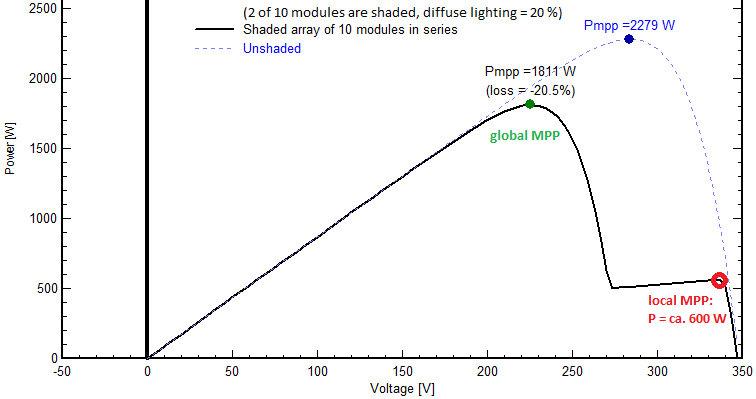
\includegraphics[width=0.95\linewidth]{MPPT/UP-curve_of_partially_shaded_solar_generator.png}
    \caption{Curva de Potencia/Voltaje de un sistema solar parcialmente obscurecido.}
\end{figure}

\subsection{¿Qué son las 3 etapas?}

El cargador MPPT de Solar Link va un paso mas allá, no solo maximizando la transferencia de potencia con pérdidas mínimas, sino que también utiliza 3 etapas diferentes para cargar la batería. Estas etapas se llaman Bulk, Absorción y Flote, las cuales le dan a la batería una carga mas profunda, aumentando su rendimiento y vida útil. \\

La fase \textbf{bulk} le entrega a la batería de manera constante la corriente máxima admitida. En esta fase, la batería se carga hasta un 80\%. Cuando se llega a un cierto voltaje (14,5V), cambia a la fase \textbf{absorción}, donde se mantiene constante este voltaje, y la bateráa llega a cargar el 20\% restante. Cuando el valor de corriente  es menor a un cierto valor (300mA), pasamos a la fase \textbf{flote}, donde se mantiene constante un voltaje menor (13,5V). Esta fase mantendrá la batería cargada cuando no esté siendo utilizada, evitando el desgaste generado en las baterías cuando no se usan por un tiempo.

\begin{figure}[H]
    \centering
    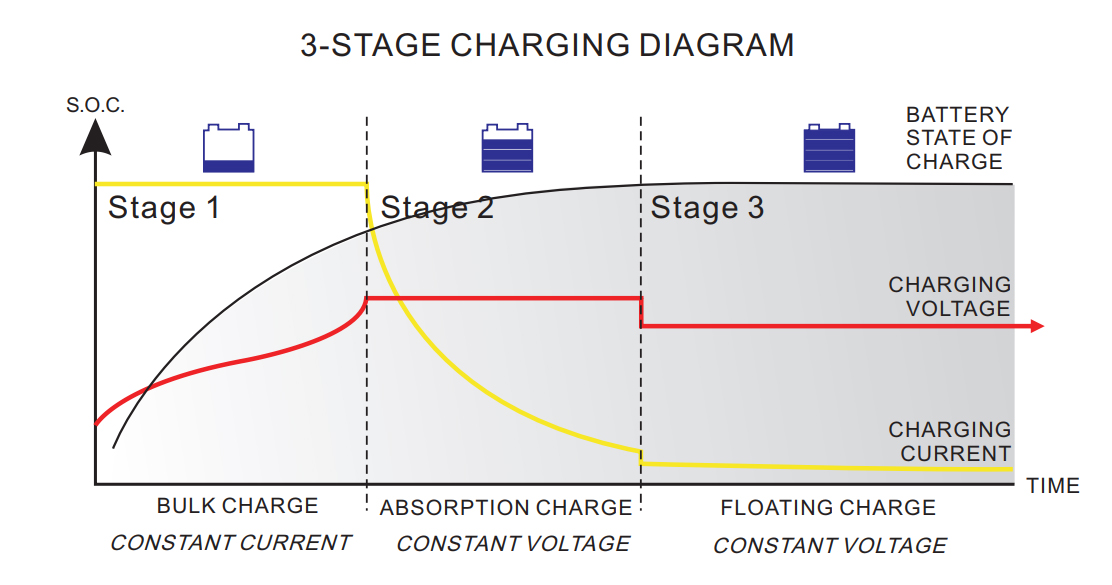
\includegraphics[width=0.95\linewidth]{MPPT/5a9f8145-6356-4504-b0b6-9d73450df4c1.jpg}
    \caption{Gráfica del voltaje, la corriente, y el porcentaje de carga de la batería en el tiempo.}
    \label{fig:grafica-carga}
\end{figure}

\subsection{Principio de funcionamiento}

\subsubsection{Convertidor Buck DC-DC}
Para convertir un voltaje de continua de entrada de mayor valor en uno de menor, existen infinidad de opciones. Por ejemplo, se podría usar un divisor resistivo, donde una resistencia disipa el voltaje que no nos interesa, pero esta opción es muy poco eficaz, porque esa energía disipada son pérdidas considerables, además en nuestro caso se necesita de un sistema que podamos controlar y variar su salida. \\

Ahi es donde entra el convertidor reductor, o convertidor Buck, que a la vez que reduce el voltaje de salida aumenta la corriente de salida, manteniendo constante la potencia. Es una clase de fuente switching, y provee una eficiencia muy alta, por encima de un 90\%. Además, controlando la señal de switching, podemos variar el voltaje de salida a voluntad.

\begin{figure}[H]
\begin{subfigure}{0.5\textwidth}
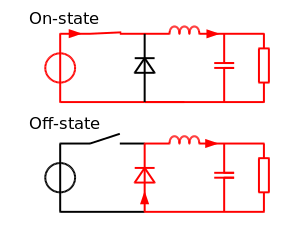
\includegraphics[width=0.9\linewidth]{MPPT/Buck_operating.svg.png} 
\caption{Las dos configuraciones de un \\convertidor Buck, On y Off.}
\label{fig:buck-1}
\end{subfigure}
\begin{subfigure}{0.5\textwidth}
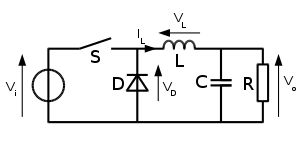
\includegraphics[width=0.9\linewidth]{MPPT/300px-Buck_conventions.svg.png}
\caption{Voltajes, corrientes y nombres de \\los componentes.}
\label{fig:buck-2}
\end{subfigure}

\caption{Convertidor Buck.}
\label{fig:image2}
\end{figure}

Para entender este circuito, se debe hacer un análisis del estado transitorio del mismo en sus dos estados, On y Off. En principio, con el estado Off, la corriente en el circuito es nula. Cuando cambia al estado On, la corriente va empezar a subir y la bobina va a generar una caída de voltaje entre sus terminales. Esta caída de voltaje provoca que el voltaje resultante en la carga sea menor. A medida que pasa el tiempo, el índice de cambio de la corriente disminuye, y el voltaje en la bobina también disminuye, aumentando el voltaje en la carga. Durante este proceso, la bobina almacena energía en forma de campo magnético. \\

Cuando el interruptor de abre de vuelta (Off), la fuente de voltaje se remueve del circuito y la corriente disminuye. Esta corriente decreciente produce una caída de voltaje en la bobina (opuesto al generado en el estado On), y ahora la bobina se convierte en una fuente de corriente. La energía almacenada en el campo magnético de la bobina suporta el flujo de corriente por la carga. Esta corriente, que fluye mientras la fuente de voltaje está desconectada, cuando se suma a la corriente que fluye en el estado On, da como resultado una corriente de salida promedio mas grande que la que entrega la fuente de voltaje.\\

\begin{figure}[H]
    \centering
    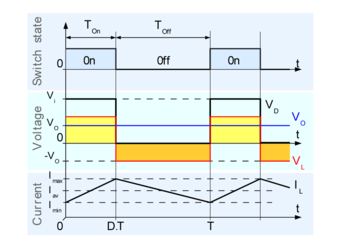
\includegraphics[width=1\linewidth]{MPPT/350px-Buck_chronogram.png}
    \caption{Gráfica en el tiempo del comportamiento de las tensiones y corrientes de un convertidor buck.}
    \label{fig:grafica-mppt}
\end{figure}

Este aumento en la corriente promedio estaría compensando la reducción en el voltaje, manteniendo idealmente la potencia entregada en la carga. Si el switch se abre mientras la corriente sigue aumentando, entonces siempre va a haber una caída de tensión sobre la bobina, por lo tanto la carga siempre tendra menos voltaje que la entrada.\\

\subsubsection{Sistema de control}
Una vez explicado el funcionamiento de la fuente reductora, ahora hay que explicar como se puede hacer para controlar ese voltaje de salida.\\

Si uno logra variar la frecuencia con la que ese switch se abre y se cierra, y al mismo tiempo medir la corriente y la tension recibida en la carga, se puede diseñar un sistema de control que, teniendo en cuenta esas variables, varíe esa frecuencia del interruptor con esas mediciones como realimentación, controlando una o la otra.\\

El sistema de control que utilizamos es un control proporcional integral, o PI, siendo la aplicación de un control proporcional y uno integral al mismo tiempo.\\

La parte proporcional de un control es el producto entre la señal de error ($e(t)$) y la constante proporcional ($K_{p}$). Variando ($K_{p}$) se cambia la velocidad del control. Pero solo con un control proporcional se tiene error en régimen permanente, ya que este tipo de control requiere de error para entregar señal de control. La fórmula matemática que responde a esto es:\\
\begin{equation}
    P_{sal}=K_{p} e(t)
\end{equation}\\

\begin{figure}[H]
    \centering
    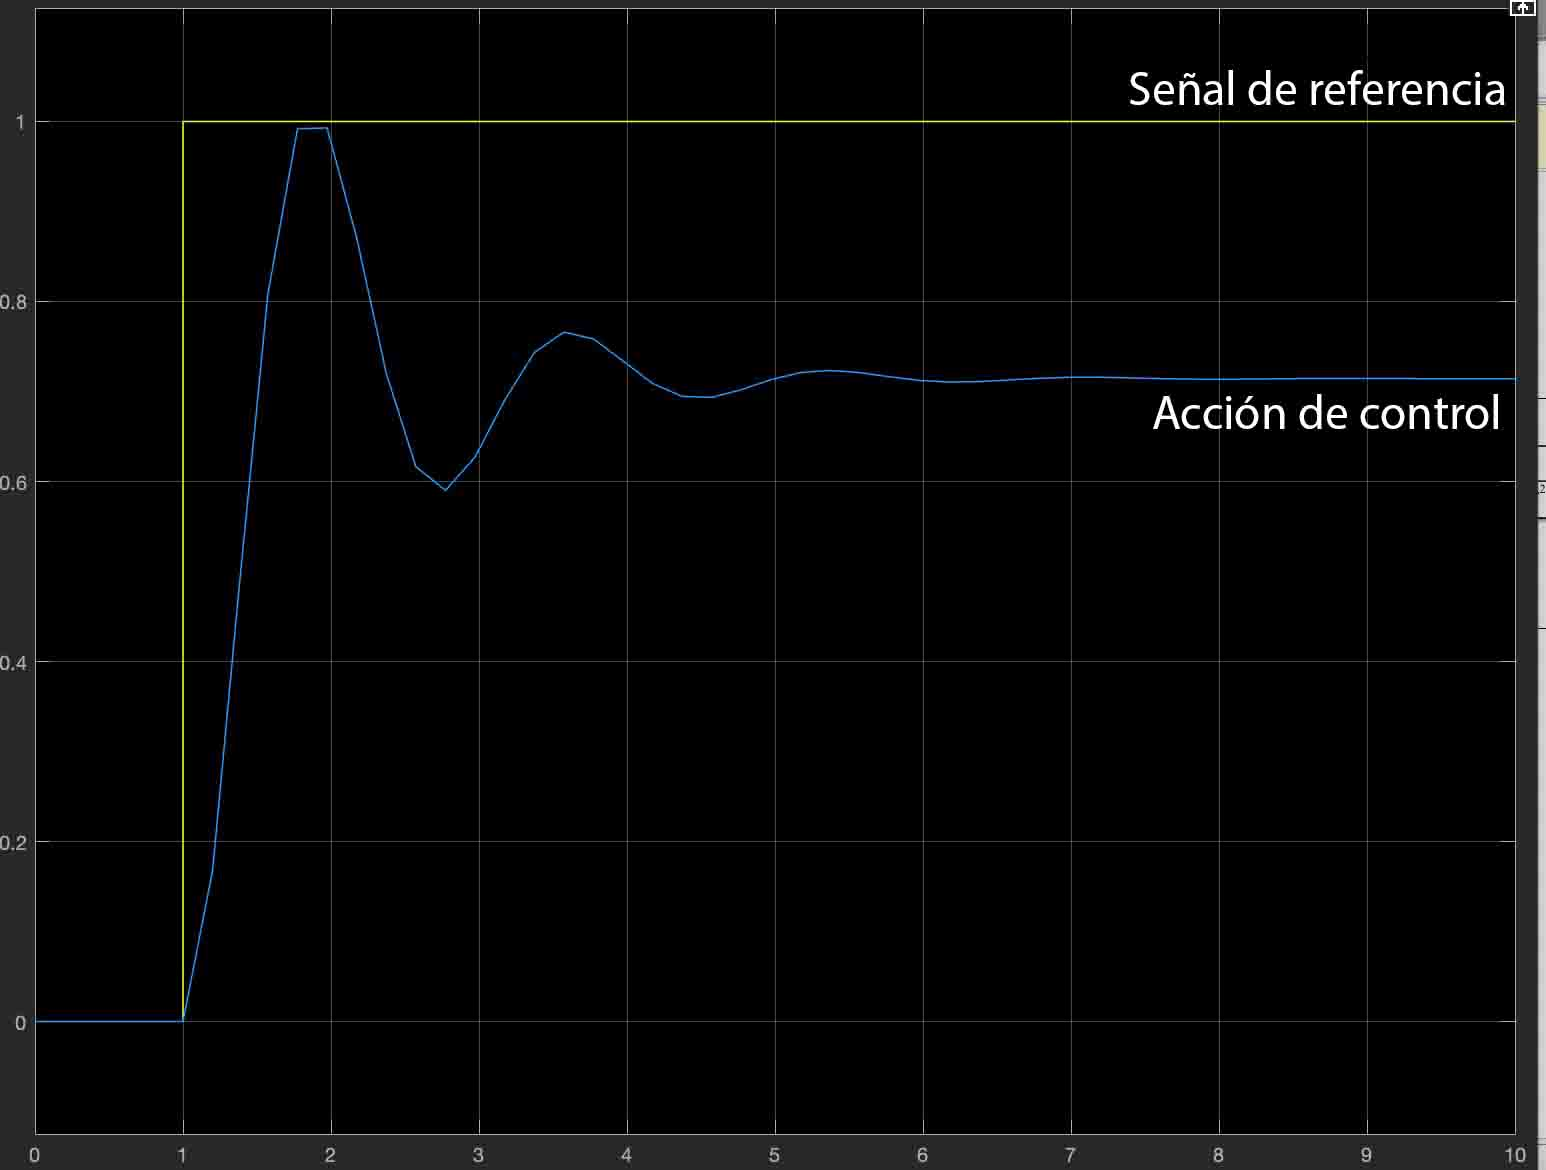
\includegraphics[width=0.7\linewidth]{MPPT/Imagen 15-10-23 a las 14.52.JPG}
    \caption{Respuesta de un control proporcional.}
    \label{fig:proporcional}
\end{figure}

La parte integral del control actua cuando hay una desviación entre la variable y el punto de consigna, integrando esta desviación en el tiempo. El error es integrado, lo cual tiene la función de promediarlo o sumarlo por un período determinado, y luego se multiplica por una constante $K_{i}$. Elimina el error de estado estacionario, logrando seguimiento perfecto de la señal de referencia. La fórmula matemática que responde a esto es:\\

\begin{equation}
    I_{sal} = K_{i} \int e(t) dt
\end{equation}


\begin{figure}[H]
    \centering
    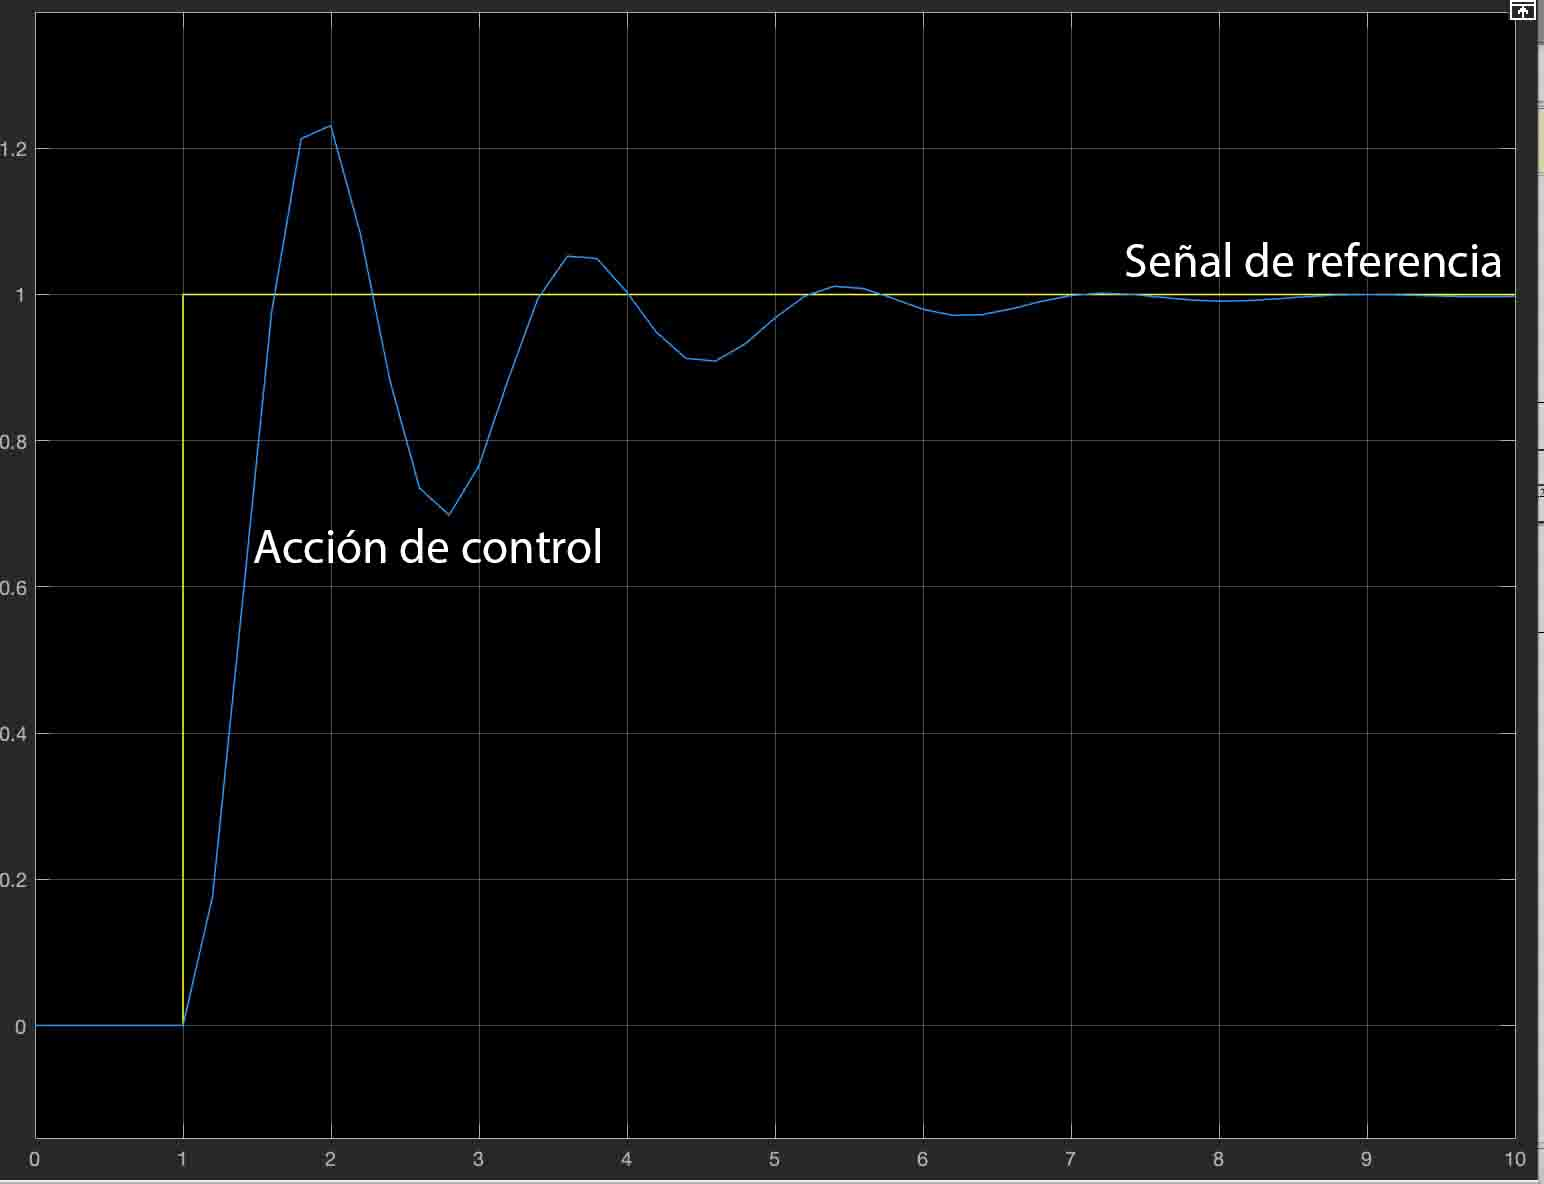
\includegraphics[width=0.7\linewidth]{MPPT/Imagen 15-10-23 a las 14.53.JPG}
    \caption{Respuesta de un control integral.}
    \label{fig:integral}
\end{figure}

Como tenemos 3 etapas de carga, donde en una la corriente es constante, y en las otras dos el voltaje lo es, vamos a necesitar controlar esas dos variables.\\

En la etapa bulk, se tendrá en cuenta el parámetro de corriente de salida y se controlará para mantenerla en un valor constante estipulado por el fabricante de la batería. En esta etapa, el voltaje será una consecuencia, y simplemente se monitorea que su valor sea menor a la tension de absorción. Si llega a este valor (tensión de absorcion), se termina la etapa bulk, y comienza la de absorción.\\

En la etapa de absorción, al contrario que la anterior, se controlará el voltaje de salida, dejando la corriente como una consecuencia. El valor de la corriente irá disminuyendo, hasta llegar a un mínimo llamado corriente de flote, donde comenzará la etapa de flote.\\

En la etapa de flote, se sigue controlando el voltaje, en este caso menor, y la corriente sigue siendo una consecuencia. En este estado se considera que la batería ya esta cargada.\\

Si la corriente de carga comienza a aumentar, es porque la batería se está utilizando, y por lo tanto está siendo descargada. Ahí es cuando se reinicia el ciclo, y empieza a correr de nuevo la etapa bulk.\\

\subsection{Realización}

\subsubsection{Hardware}

\begin{figure}[H]
    \centering
    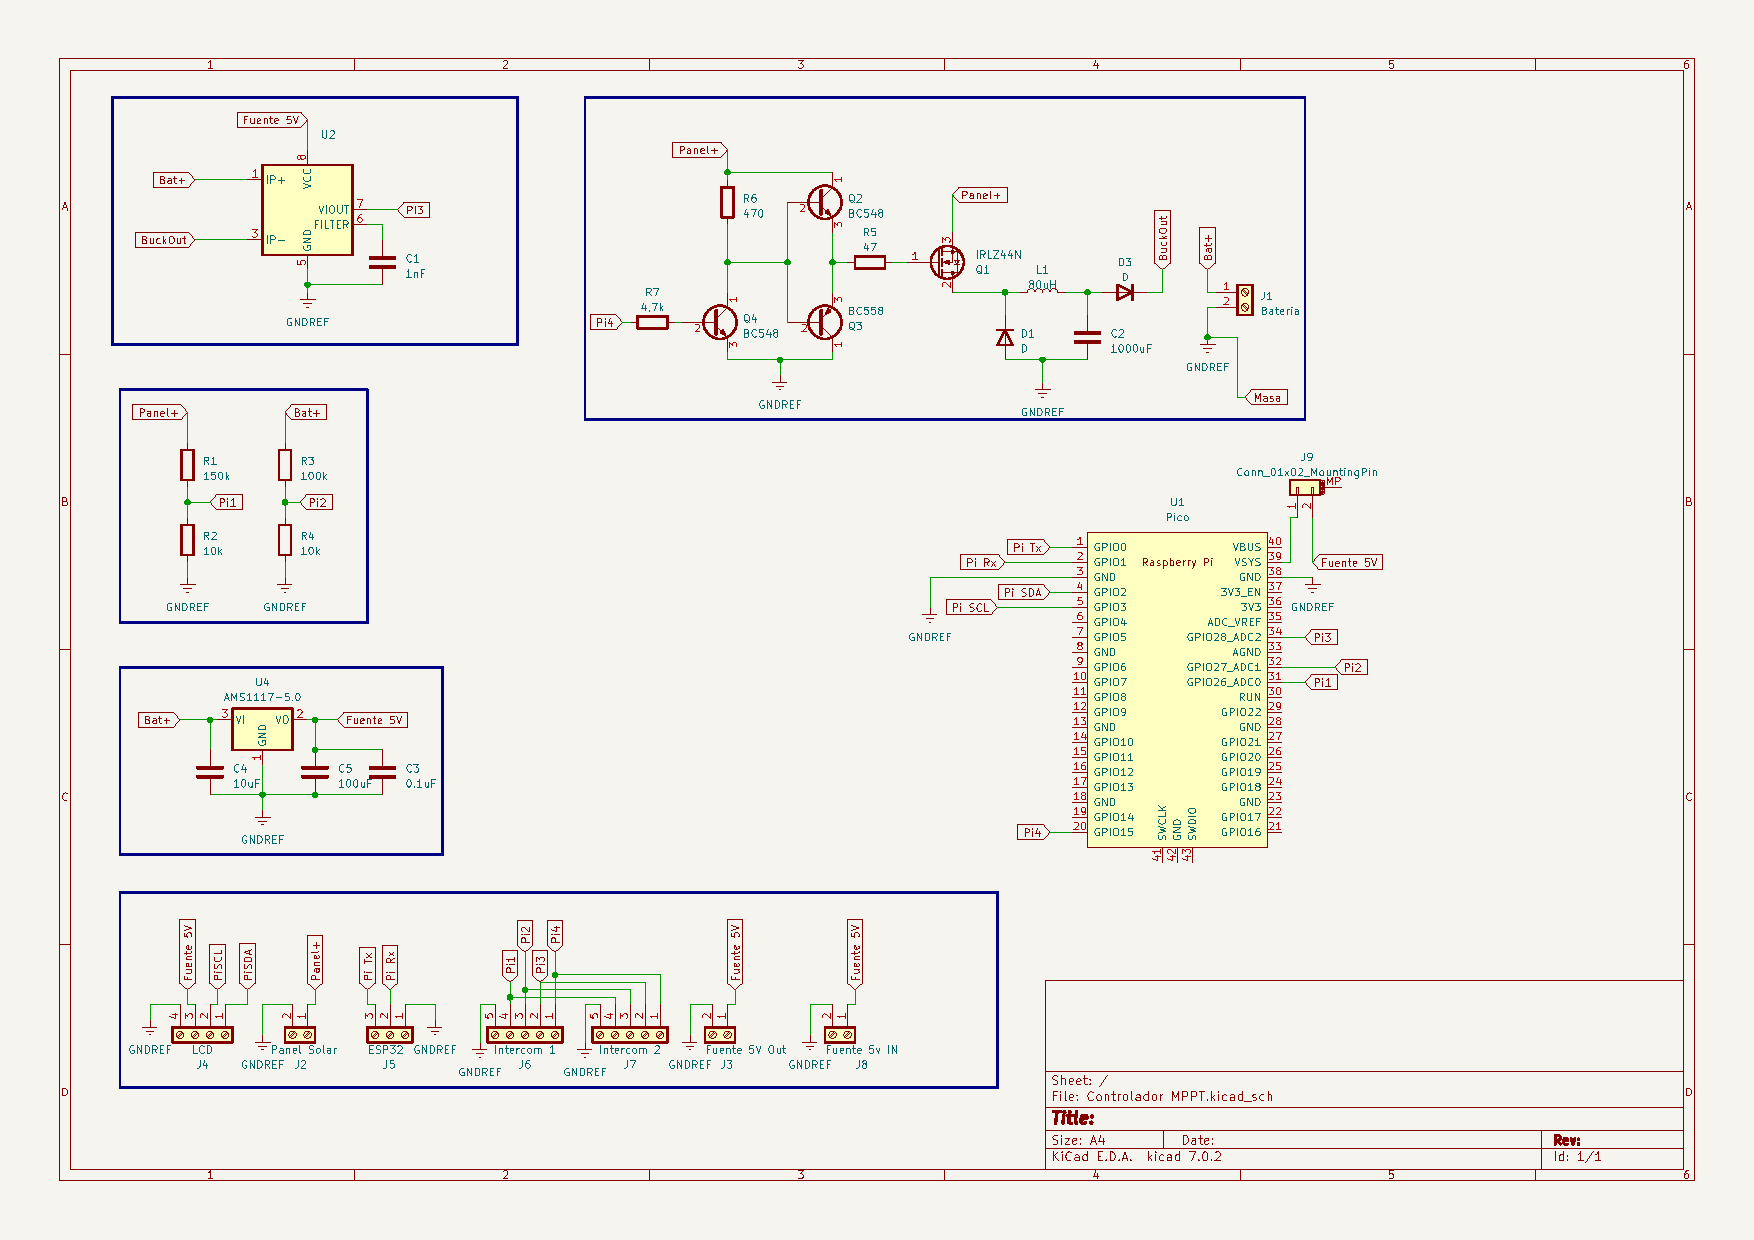
\includegraphics[width=1\linewidth]{MPPT/Controlador MPPT.pdf}
    \caption{Circuito MPPT completo.}
    \label{fig:enter-label}
\end{figure}

\begin{wrapfigure}{l}{0.35\textwidth}
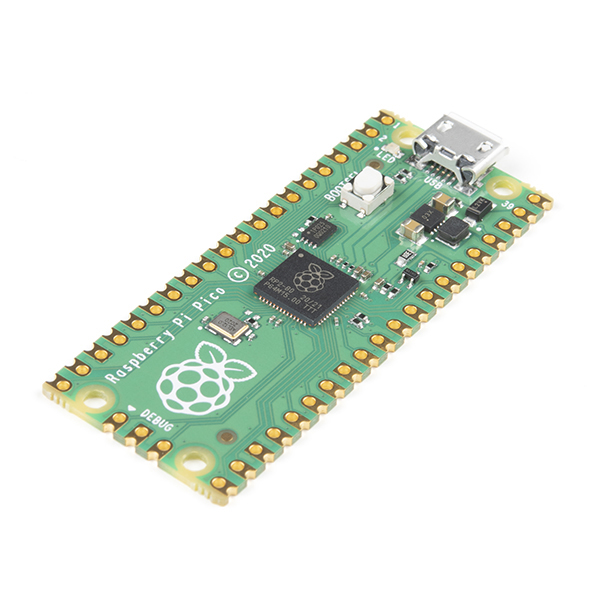
\includegraphics[width=0.9\linewidth]{MPPT/17829-Raspberry_Pi_Pico-01.jpg} 
\caption{Raspberry Pi Pico}
\label{fig:wrapfig}
\end{wrapfigure}

Para realizar este cargador, utilizamos una Raspberry Pi Pico como controlador principal, encargada de leer todos los parámetros, controlar el voltaje o la corriente de salida, y comunicarse con el módulo Solar Link para informar los parámetros medidos.\\

\begin{wrapfigure}{r}{0.25\textwidth}
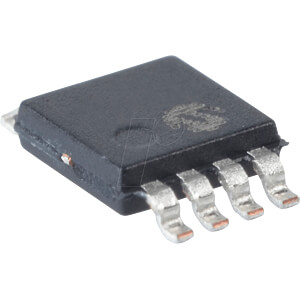
\includegraphics[width=0.9\linewidth]{MPPT/acs712.jpg} 
\caption{Sensor de corriente ACS712}
\label{fig:wrapfig}
\end{wrapfigure}

Para medir la corriente utilizamos el sensor ACS712xLCTR-20A, el cual es un sensor de efecto Hall que nos permite medir corrientes positivas y negativas, y nos devuelve esta información entre 0V y 5V. Esto quiere decir que -20A son 0V, 0A son 2,5V, y 20A son 5V. Esta información es procesada por un ADC de la Raspberry Pi Pico.\\

Para medir las tensiones tanto de entrada como de salida simplemente utilizamos divisores resistivos, los cuales nos devuelven voltajes proporcionales reducidos, tambien procesados por los otros dos ADCs de la Raspberry Pi Pico. Para la conversion simplemente se tiene en cuenta la relacion de las resistencias.\\

Para la alimentación del circuito aprovechamos el voltaje de entrada de la batería, donde conectamos una fuente Step Down que regula el voltaje de alimentacion de la Raspberry Pi Pico en 5V. Esto quiere decir que una vez que se conecta la batería para comenzar la carga, el circuito ya se encuentra alimentado por energía verde para funcionar.\\

Para mostrar los datos medidos en tiempo real, utilizamos un LCD de 20x04, donde entran se pueden mostrar sin problemas estos datos. El cargador indica el voltaje de entrada, voltaje de salida, corriente de salida, \% de PWM utilizado, y fase de carga.\\

\begin{figure}[H]
    \centering
    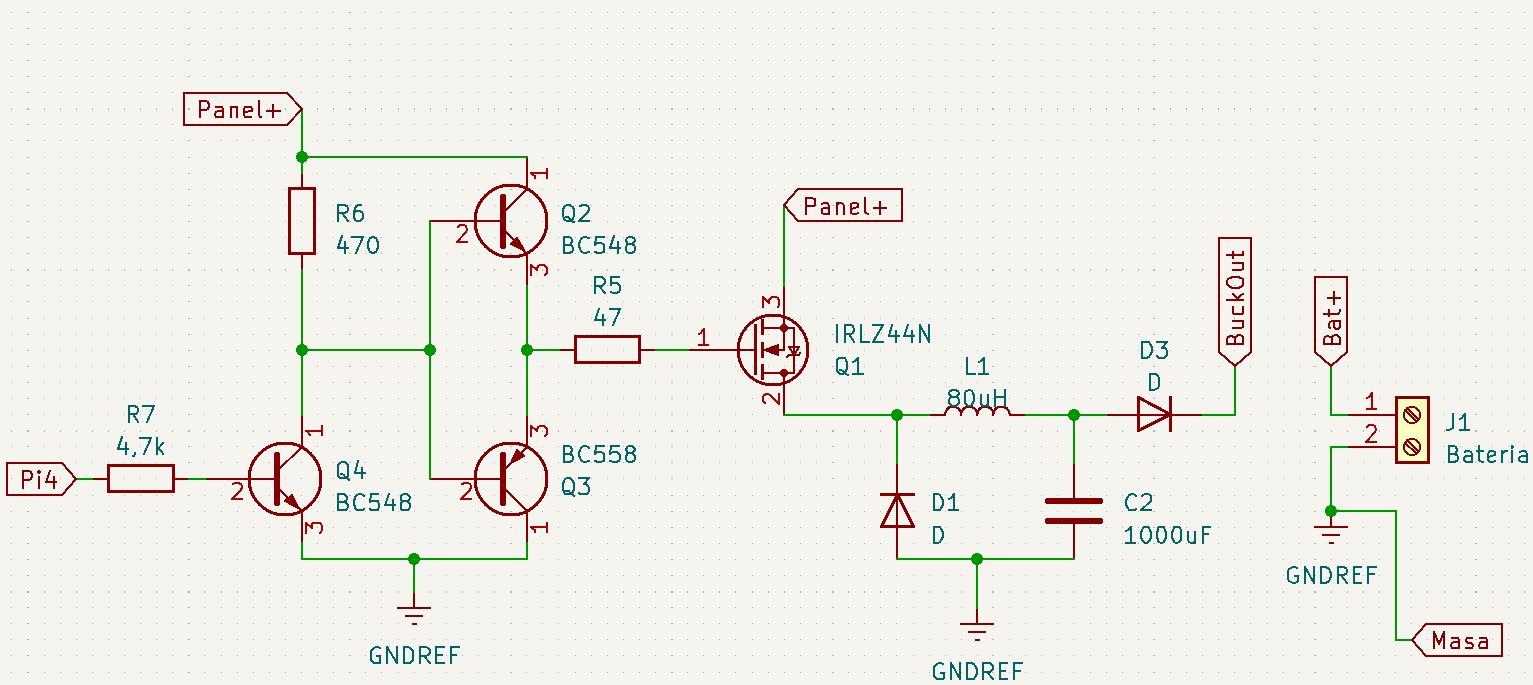
\includegraphics[width=1\linewidth]{MPPT/Screenshot_7.png}
    \caption{Circuito MPPT.}
    \label{fig:circuito MPPT}
\end{figure}

En el circuito MPPT, la única diferencia con el teórico es el interruptor. Nuestro interruptor es un MOSFET canal P \href{https://www.alldatasheet.es/datasheet-pdf/pdf/683453/KERSEMI/IRF4905.html}{IRF4905}, que resiste hasta 70A de corriente. Es necesaria la utilización de un MOSFET canal P porque la carga del mismo tiene que estar entre Drain y Masa, mientras que la carga de un canal N tiene que estar entre la alimentación y Source, algo que en nuestro diseño resultó inconveniente.\\

Para conmutar este MOSFET con la Raspberry Pi Pico, no solo fue necesaria la utilización de un transistor NPN, sino tambien la de un circuito totem pole. \\

\begin{figure}[H]
    \centering
    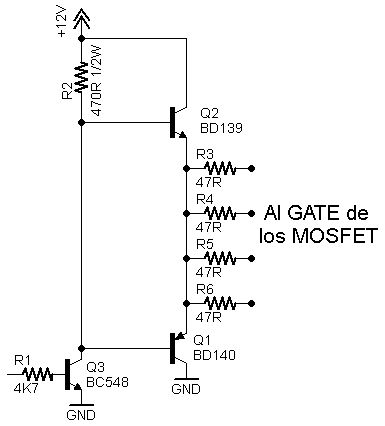
\includegraphics[width=0.8\linewidth]{MPPT/Imagen de WhatsApp 2023-10-11 a las 20.57.02_7faa2d47.jpg}
    \caption{Circuito Totem Pole.}
    \label{fig:enter-label}
\end{figure}

Un circuito totem pole consta de 2 transistores, un PNP y un NPN, uno arriba del otro, con sus bases interconectadas. Esto nos permite conmutar el MOSFET sin problemas, porque admite corrientes en ambos sentidos, tanto positivas como negativas. Esto es necesario porque un MOSFET necesita ambos sentidos de corrientes. Para entrar en estado de corte, necesita una corriente positiva en el Gate, y para volver al estado de saturación, por las características capacitivas del mismo, genera una corriente negativa.\\

Para el cálculo del inductor, se realizó el siguiente procedimiento:

Fijándose en la figura \ref{fig:grafica-mppt}, el aumento de la corriente en la bobina queda:

\begin{equation}
\frac{di_L(t)}{dt} = \frac{V_L(t)}{L} = \frac{V_i - V_o}{L}    
\end{equation}

y análogamente el descenso de corriente es:

\begin{equation}
\frac{di_L(t)}{dt} = \frac{V_L(t)}{L} = \frac{-V_o}{L}    
\end{equation}

Como toda la energía que se almacena en la bobina durante el primer estado se transfiere durante el segundo, la energía del inductor al final del periodo de conmutación ($T_S$) es igual en $t = 0$ y en $t = T_S$.\\

Por lo tanto, la tensión media en la bobina $\langle V_L \rangle$ en régimen permanente es nula, es decir, existe una igualdad en las áreas.

\begin{equation}
    \langle V_L \rangle = \frac{1}{T_s}\int_{T_s} V_L dt = 0
\end{equation}

Aplicando la ecuación se obtiene:

\begin{equation}
    (V_i - V_o) \cdot DT_s - V_o \cdot (T_s - DT_s) = 0
\end{equation}

Donde D es un número adimensional, entre 0 y 1, denominado ciclo de trabajo. Siendo que este no puede ser mayor a 1, se cumple $V_o \leq V_i$, por tanto solo se podrá reducir la tensión.

\begin{equation}
    V_o = D \cdot V_i
    \label{eq:D}
\end{equation}

La corriente media que circula por la bobina, con un D del 10\% (peor condición posible):\\

\begin{equation}
    I_L > \frac{I_{Lmax}}{10} = 2
\end{equation}



\begin{equation}
    \frac{\Delta I_L}{2} < 2 \Rightarrow \Delta I_L < 4
\end{equation}\\

Para calcular la bobina, se utiliza la siguiente fórmula:\\

\begin{equation}
    \frac{V_i - V_o}{L} \cdot D \cdot T_S < 4
\end{equation}\\

Reemplazando D por la equivalencia obtenida en la fórmula \ref{eq:D}, queda:\\

\begin{equation}
    L \geq \frac{V_o(1-\frac{V_o}{V_i})\cdot T_S}{4}
\end{equation}

Siendo
\[V_i [12V-36V]\]
\[V_o [12V-15V]\]
\[T_S = 32 \cdot 10^{-6} S  = 32KHz\]\\

El máximo de esta función queda definido por los máximos valores de tensión de entrada y tensión de salida, por lo tanto:\\

\begin{equation}
    L \geq \frac{15 \cdot (1-\frac{15}{36}) \cdot 32 \cdot 10^{-6}}{4}
\end{equation}

Entonces \[L \geq 68uH\]\\

La bobina utilizada en el circuito posee un valor de \textbf{$83uH$}, la cual cumple con la condición anterior.\\

Para el cálculo del capacitor correspondiente, se realizó el siguiente procedimiento:\\

Cálculo para el ripple del capacitor de un 1\%: 

\begin{equation}
    \Delta V_o = 1\% \cdot 15V = 0,15V
\end{equation}

La fórmula utilizada para obtener el valor del capacitor es la siguiente:\\

\begin{equation}
    \Delta V_o = \frac{V_o \cdot (1-\frac{V_o}{V_i})}{8 \cdot L \cdot C \cdot F^2}
\end{equation}\\

Despejando, se obtiene:\\

\begin{equation}
    C \geq \frac{V_o \cdot  (1 - \frac{V_o}{V_i})}{8 \cdot L \cdot \Delta V_o \cdot F^2}
\end{equation}\\

Con los valores ya calculados, se reemplazan los parámetros:\\

\begin{equation}
    C \geq \frac{15V \cdot (1 - \frac{15V}{36V})}{8 \cdot 83uH \cdot 32KHz^2}
\end{equation}

Entonces \[C \geq 12uF\]\\

Para evitar resonancias, se estima que la frecuencia de resonancia tiene que estar 10 veces por debajo de la frecuencia en la que se trabaja. Por esto:\\

\begin{equation}
    \frac{F_S}{10} = \frac{1}{\sqrt{L \cdot C}}
\end{equation}

Despejando, queda:\\

\begin{equation}
    C = \frac{10^2}{32KHz^2 \cdot 83uH} \simeq 1100uF
\end{equation}\\

Por lo tanto, en el circuito final se utilizó un capacitor de \textbf{$1000uF$}

\subsubsection{Software}

El sistema MPPT fue programado íntegramente con el lenguaje C sobre la Raspberry Pi Pico. \\

El microcontrolador lee las señales del divisor de tensión que caerá sobre sus ADC y, mediante una lógica dependiente de la relación entre las resistencias del divisor de tensión, el código interpreta estas señales para saber el valor deseado (ya sea corriente o votaje). Referirse a Listing \ref{Listing 1}  o Listing \ref{Listing 2}\\

Ya sabiendo los valores que se tienen que medir, se compararán con los valores definidos para el cambio de lógica. Así se define en que modo de carga estará el MPPT. Por ejemplo, para el cambio entre BULK y ABSORTION, el voltaje de la batería deberá ser mayor al voltaje máximo definido del modo BULK. Referirse a Listing \ref{Listing 3}, pag 25\\

Tambien, cada vez que se define el modo y los valores de cada variable, se los mostrara en un display LCD. \\

Cada modo tiene su propia lógica para manejar el PWM que regula la tensión y corriente que le llega a la batería. En el modo BULK, primero se calcula el error entre la medicion actual y la deseada, luego se ve si la corriente que le llega a la batería es mayor o menor a la deseada y en base a esto se controla el PWM proporcionalmente e integralmente tomando en cuenta el error (Referirse a Listing \ref{Listing 4}), pasando previamente por un saturador, asegurándose que el valor del PWM no sea ni mayor a 100\% ni menor a 0\%. Referirse a Listing \ref{Listing 5}\\

Luego de todo este proceso, el valor actual del PWM es mostrado en la pantalla del LCD. Referirse a Listing \ref{Listing 6}\\

Para la comunicación con el otro microcontrolador, se utiliza UART. Con este objetivo, la Raspberry Pi Pico realiza una interrupción cada 1 segundo, reteniendo los datos de consumo actual. Cada 60 segundos estos datos se promediarán y se guardarán en otra variable, aumentando un contador (Referirse a Listing \ref{Listing 7}). Cuando el otro micro mande una señal, se promediaran los valores guardados y se enviara un promedio de consumo. Referirse a Listing \ref{Listing 8}\\

\subsubsection{Resultado final}

El prototipo final de nuestro cargador MPPT de 3 etapas es completamente funcional, probado con paneles solares y diferentes baterías, sin presentar fallas despues de horas de funcionamiento.\\

En las pruebas realizadas, se concluyó que es un cargador muy versátil, que con cambiar unos pocos parámetros se pueden cargar todo tipo de baterías de plomo-ácido, en un tiempo razonable, y entregando una carga profunda muy saludable para la vida útil de una batería.\\

\begin{figure}[H]
    \centering
    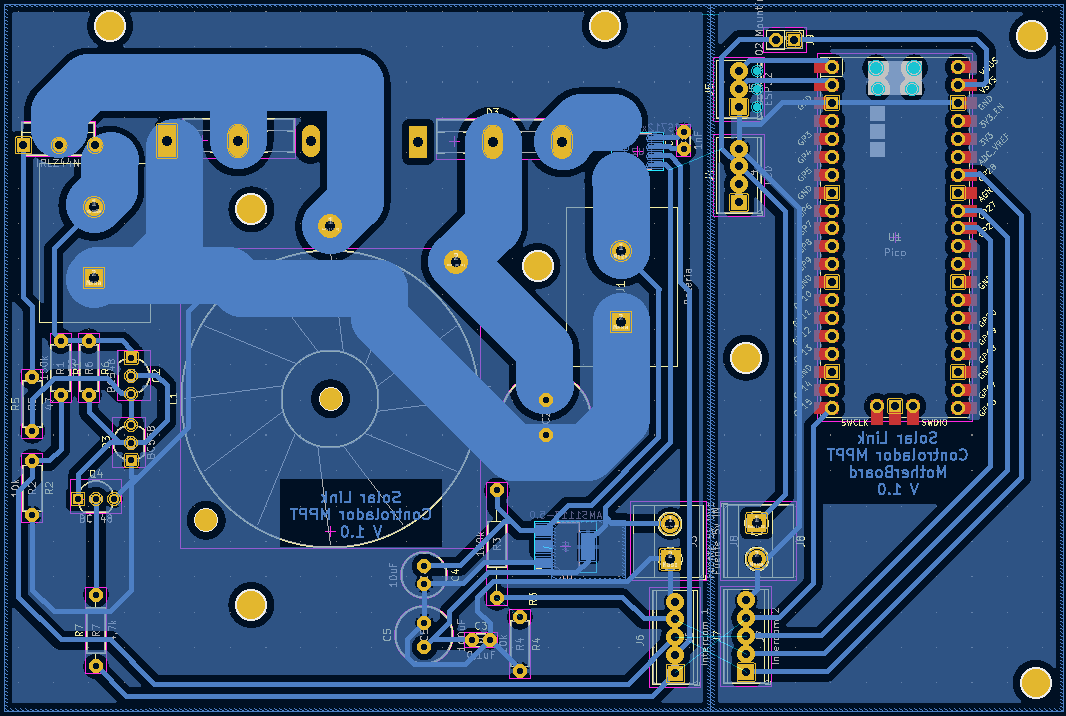
\includegraphics[width=1\linewidth]{MPPT/Screenshot_9.png}
    \caption{Diseño PCB.}
    \label{fig:PCB-MPPT}
\end{figure}

\begin{figure}[h]

\begin{subfigure}{0.5\textwidth}
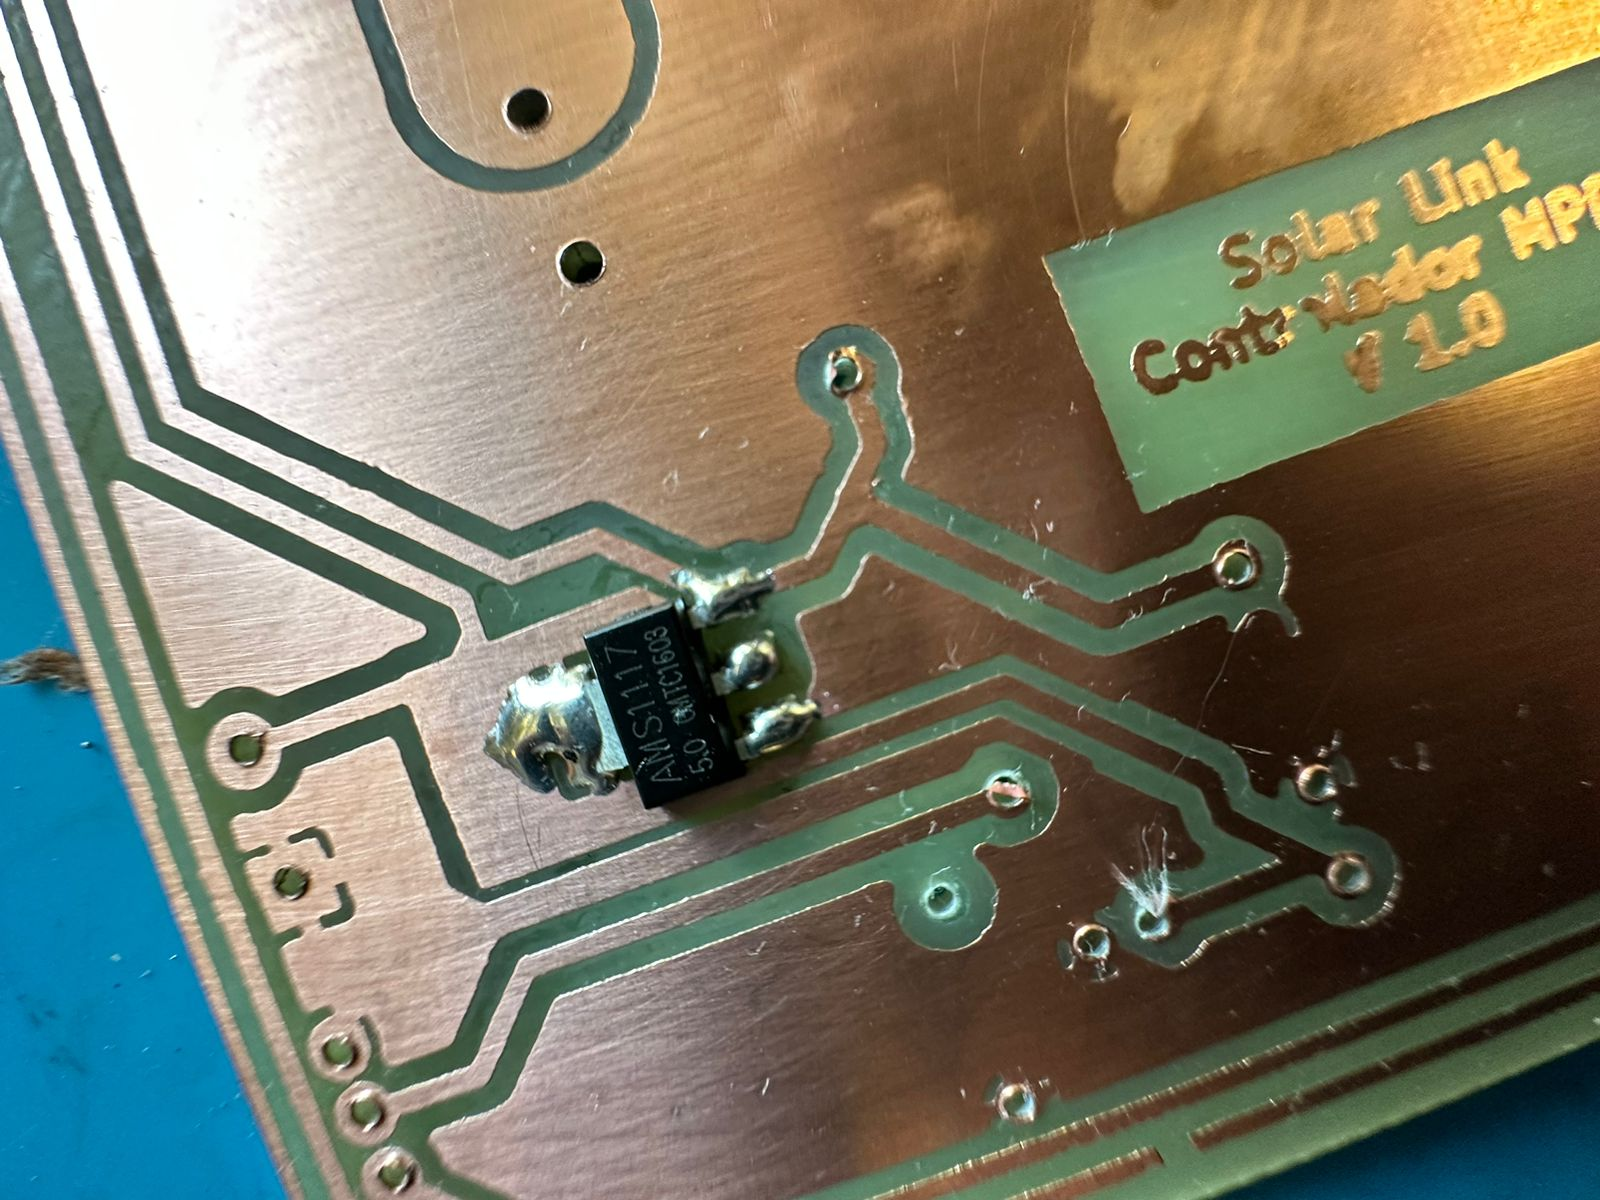
\includegraphics[width=0.9\linewidth]{MPPT/IMG_8867.JPG} 
\caption{Regulador 5V}
\label{fig:regulador12}
\end{subfigure}
\begin{subfigure}{0.5\textwidth}
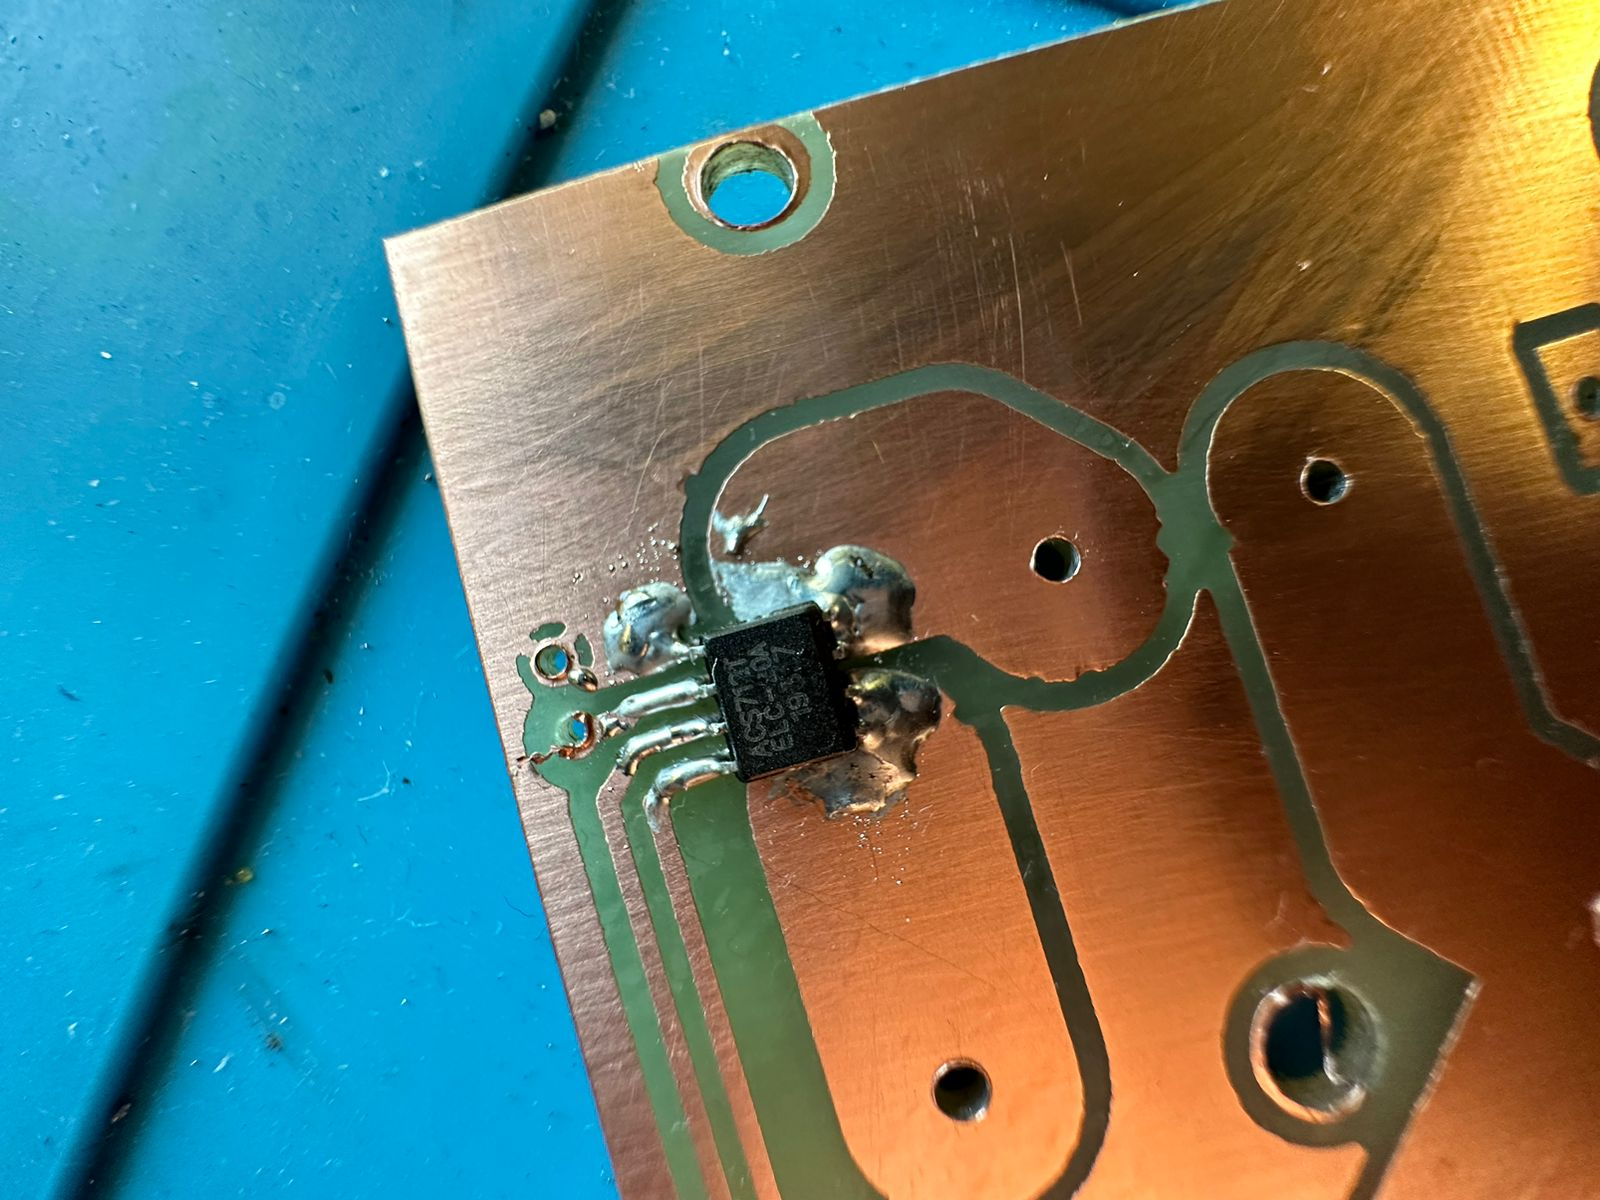
\includegraphics[width=0.9\linewidth]{MPPT/IMG_8868.JPG}
\caption{Sensor de corriente ACS712}
\label{fig:sensor-corr}
\end{subfigure}

\caption{Soladura SMD en la placa.}
\label{fig:image2}
\end{figure}

\begin{figure}[H]
    \begin{subfigure}{0.5\textwidth}
        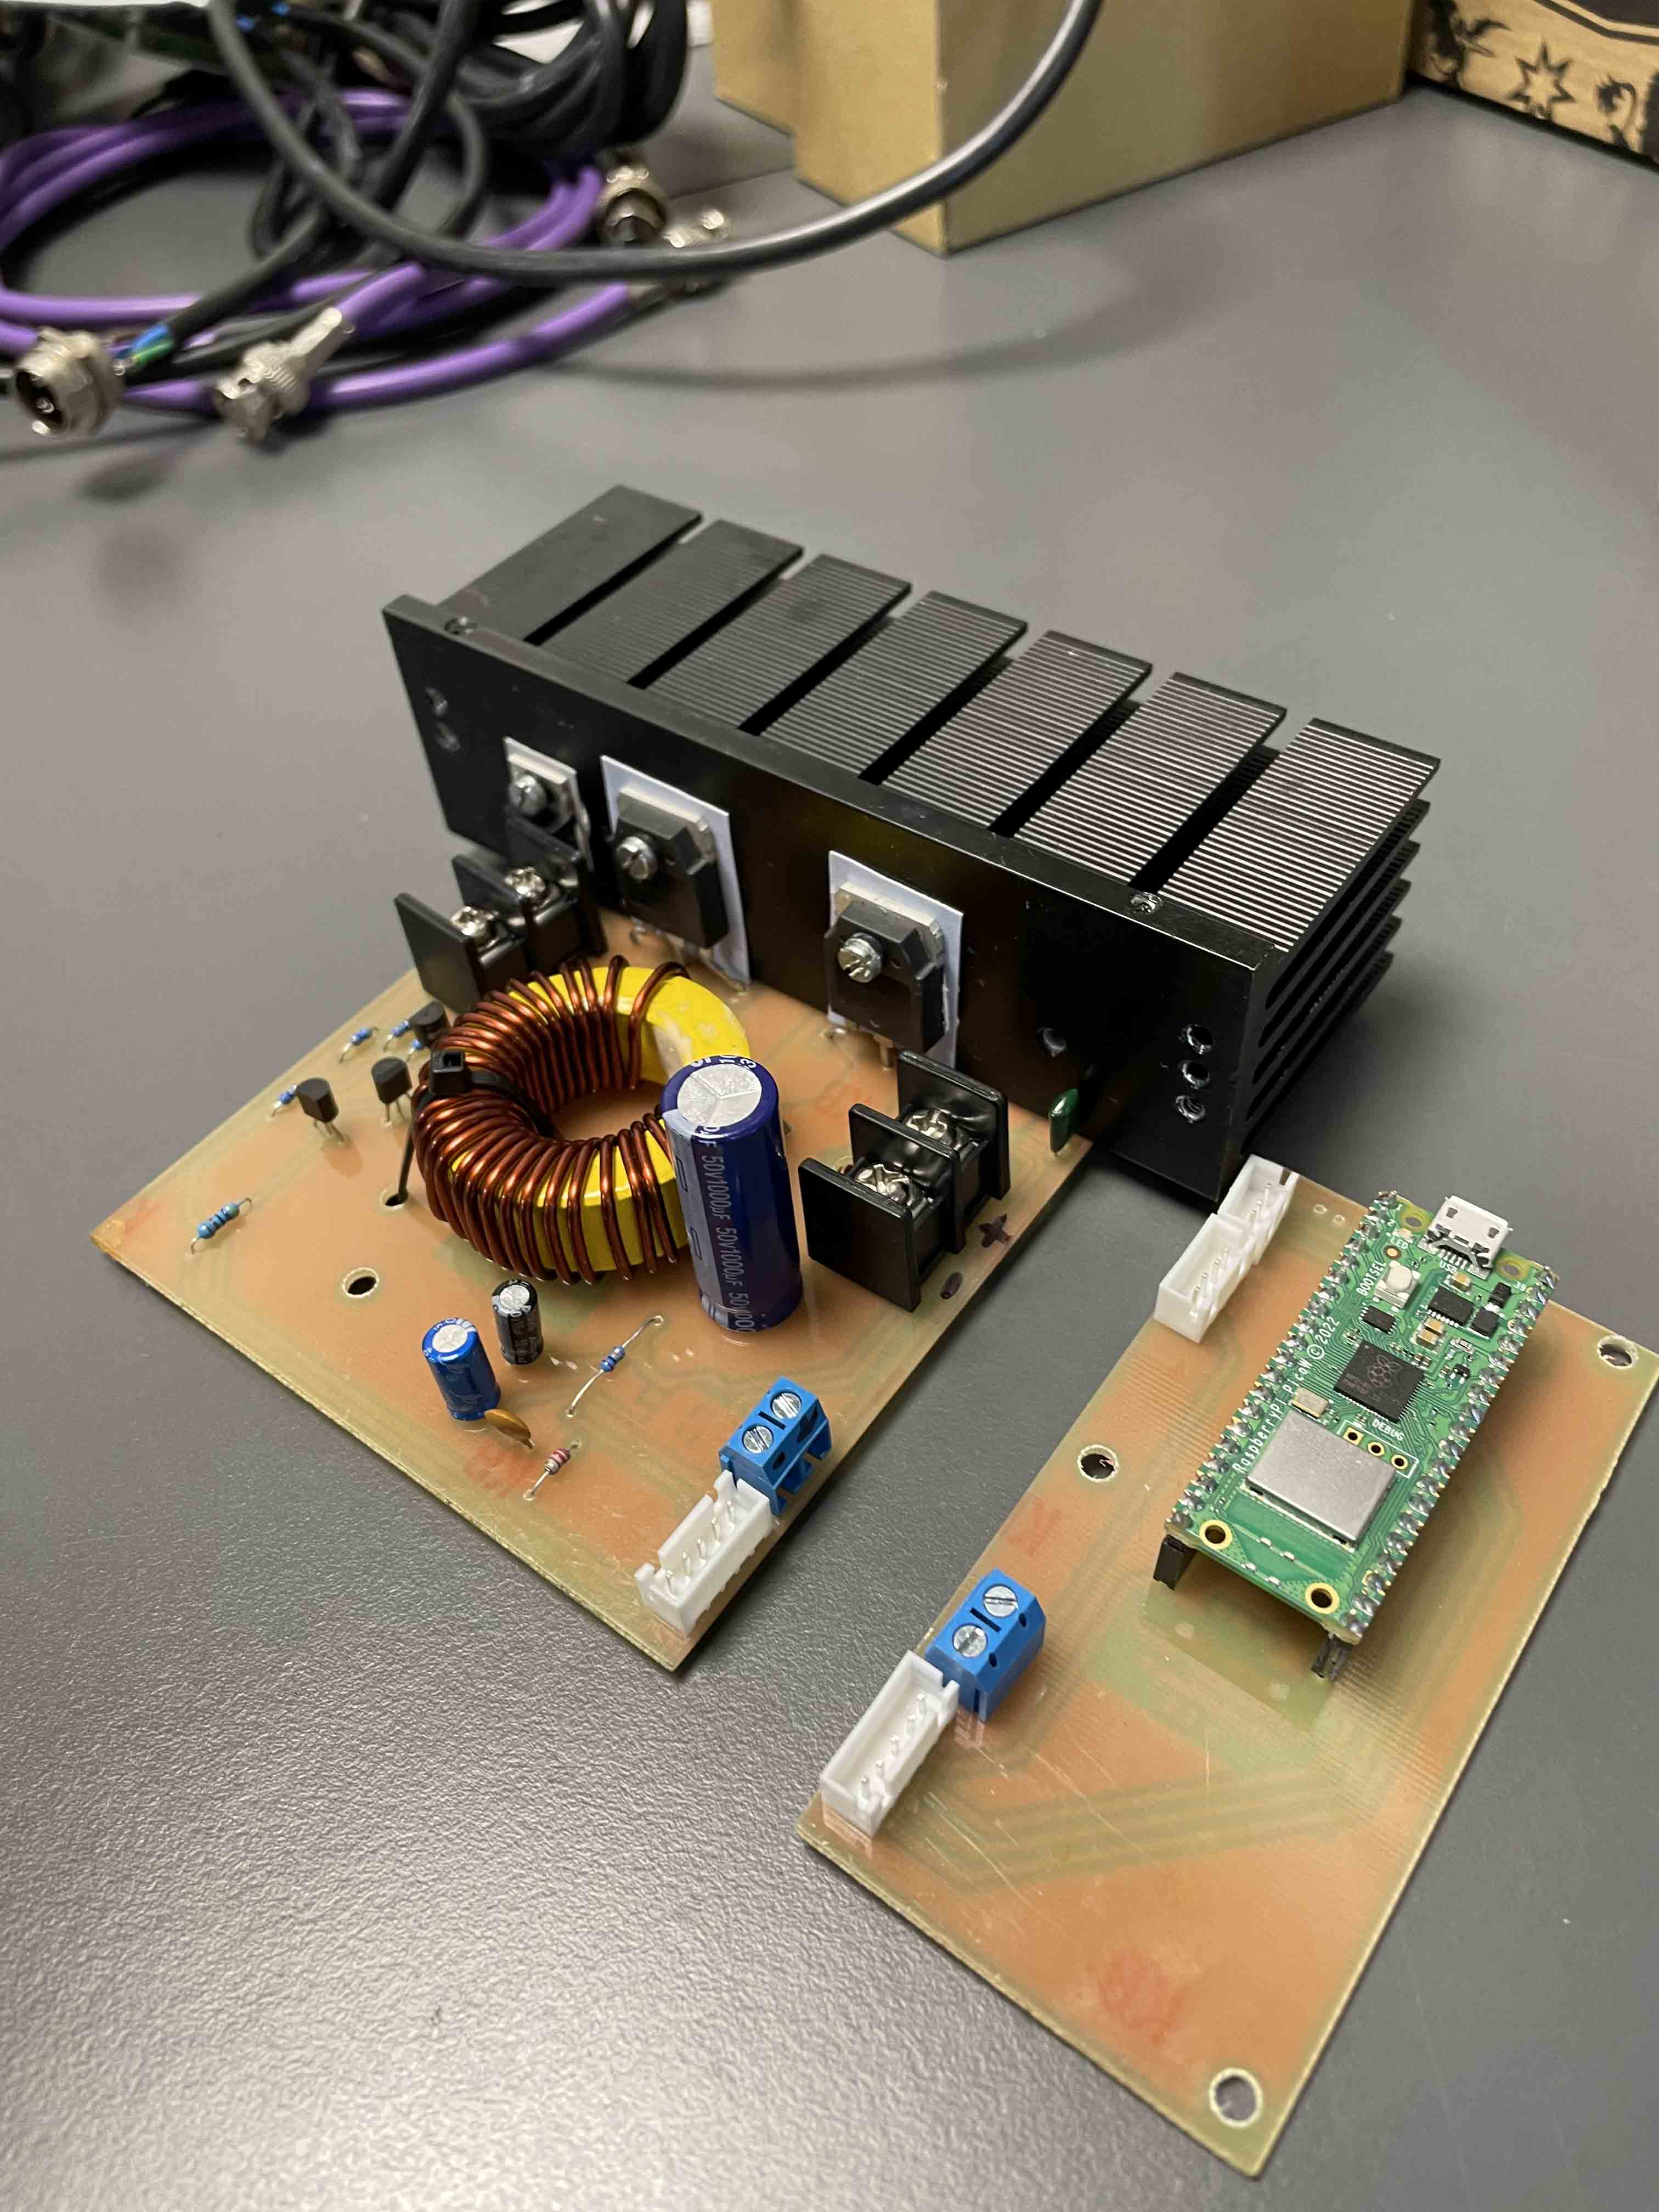
\includegraphics[width=0.9\linewidth]{MPPT/IMG_8864.jpg} 
        \caption{Plaqueta final del cargador.}
        \label{fig:subim1}
    \end{subfigure}
    \begin{subfigure}{0.5\textwidth}
        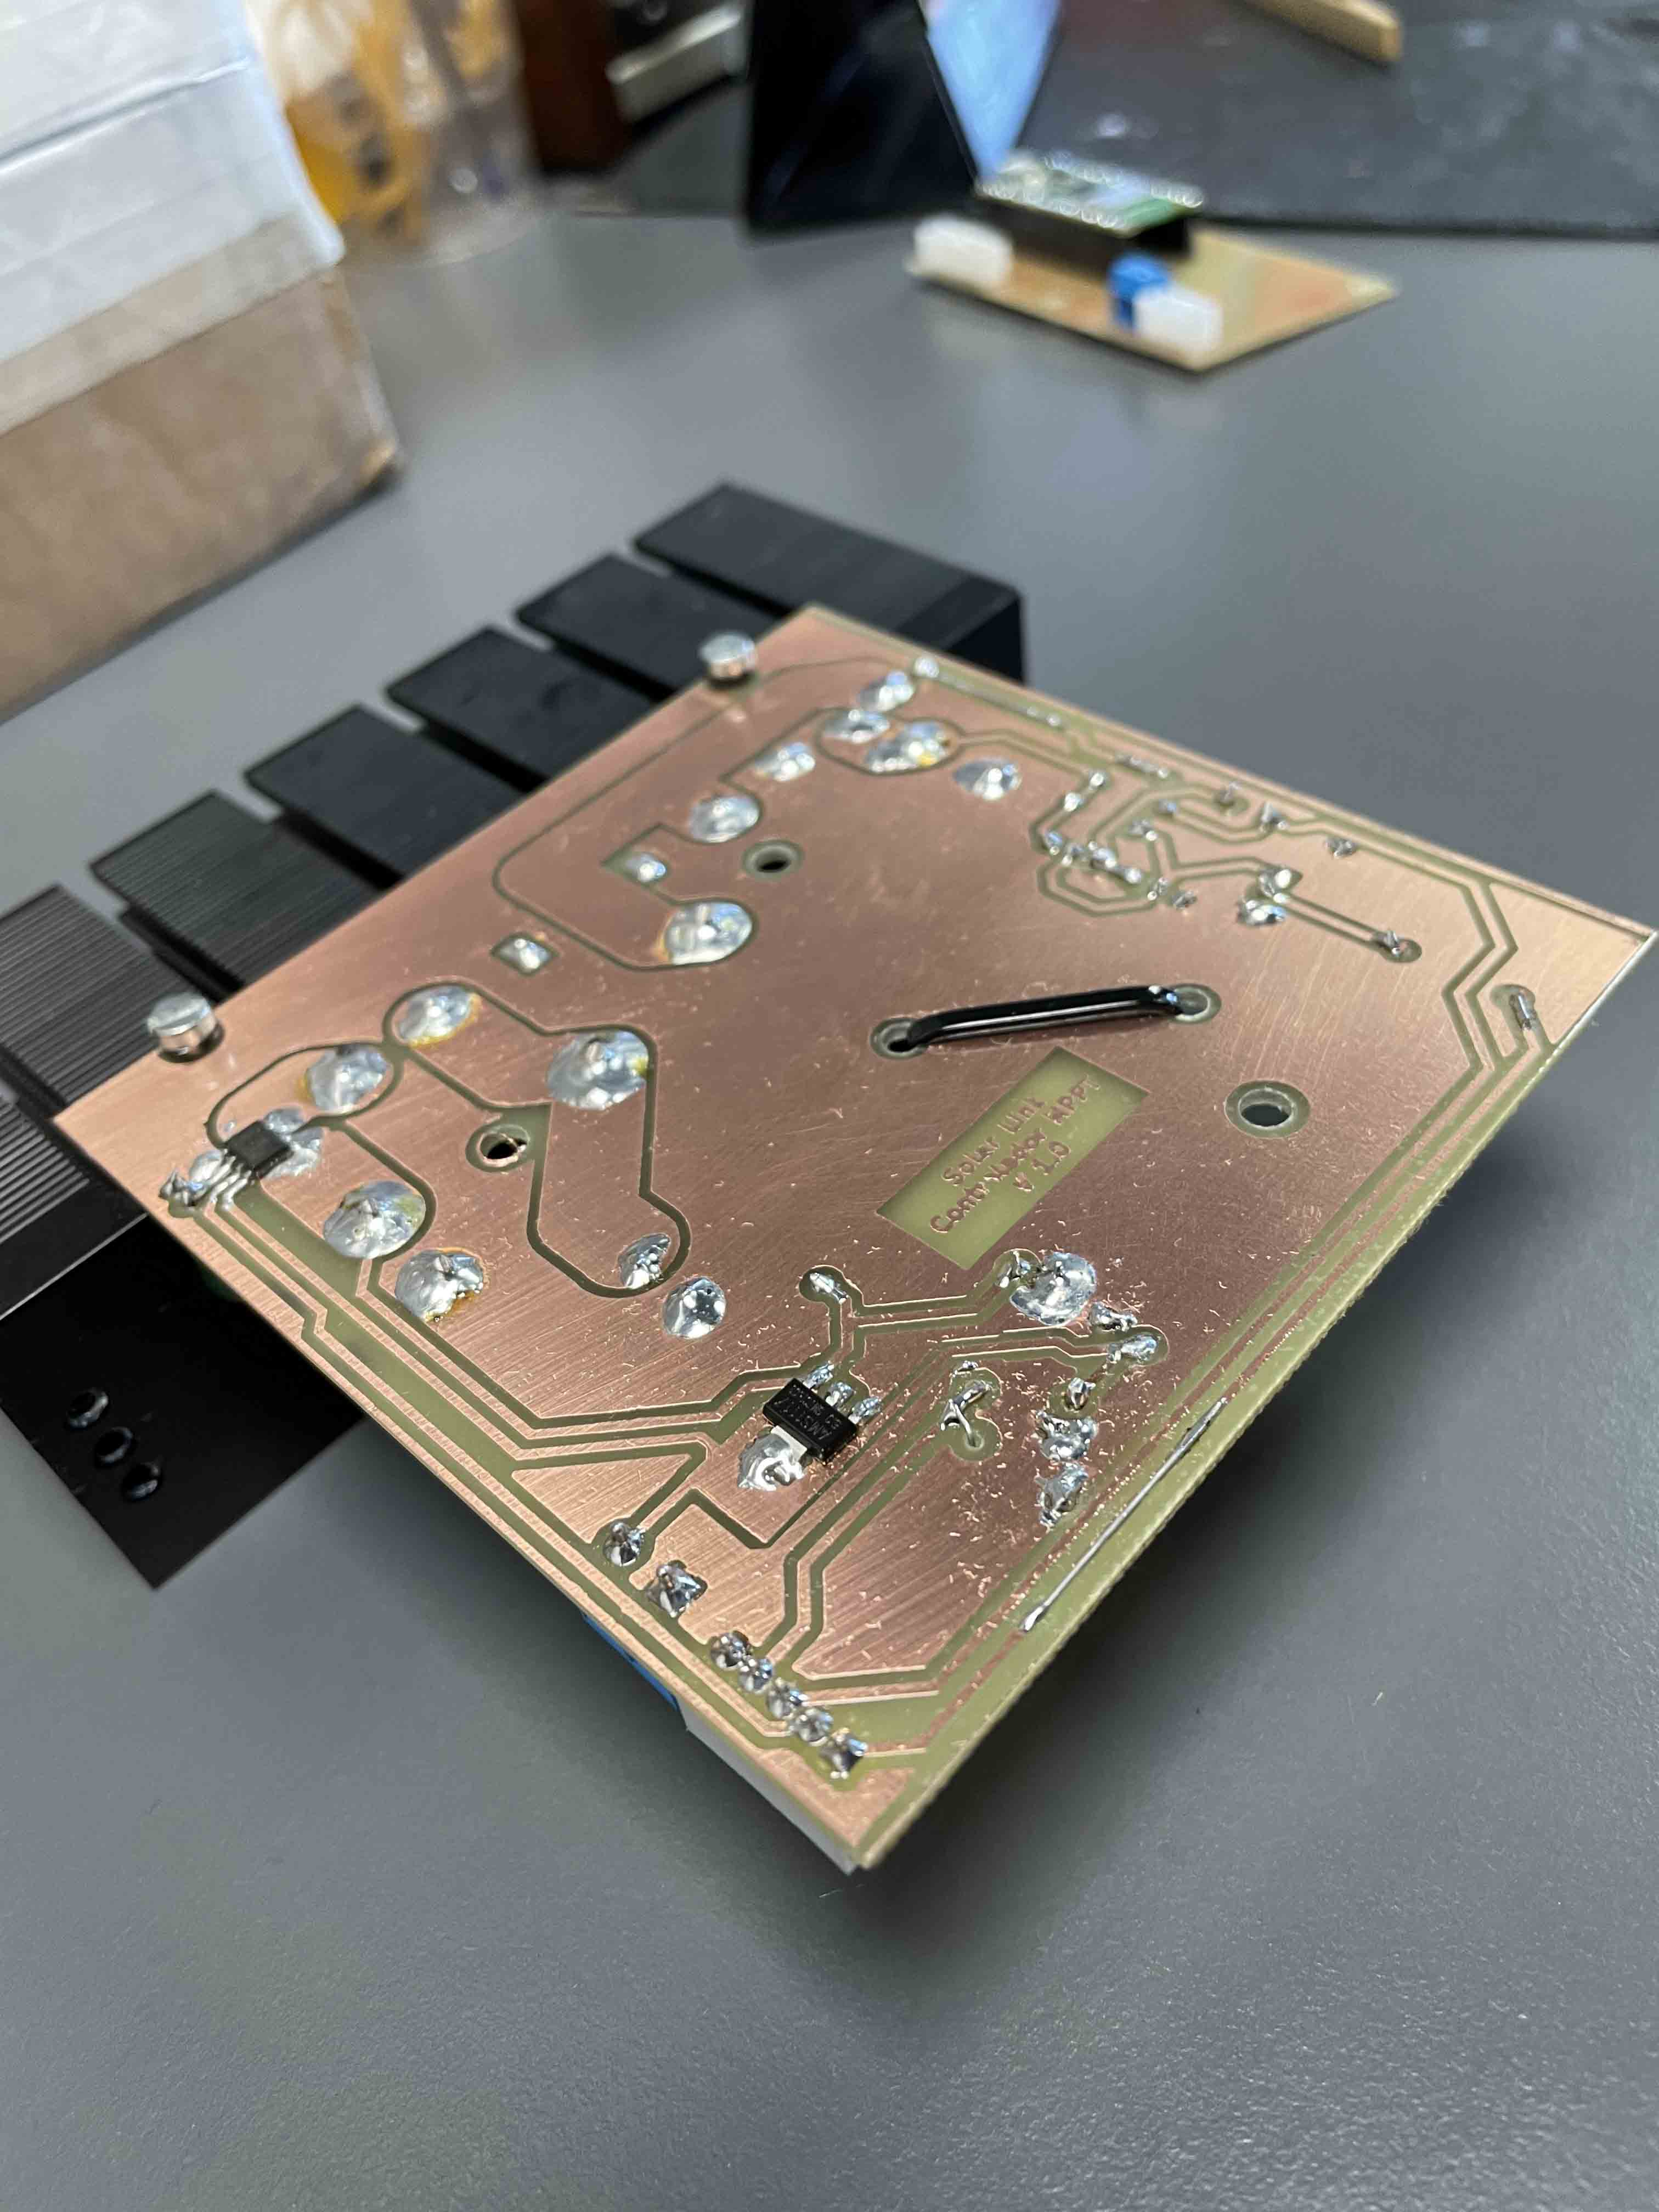
\includegraphics[width=0.9\linewidth]{MPPT/IMG_8866.jpg}
        \caption{Plaqueta final, lado inferior.}
        \label{fig:subim2}
    \end{subfigure}
\caption{Plaquetas finales cargador MPPT.}
\end{figure}

\begin{figure}[H]
    \begin{subfigure}{0.5\textwidth}
        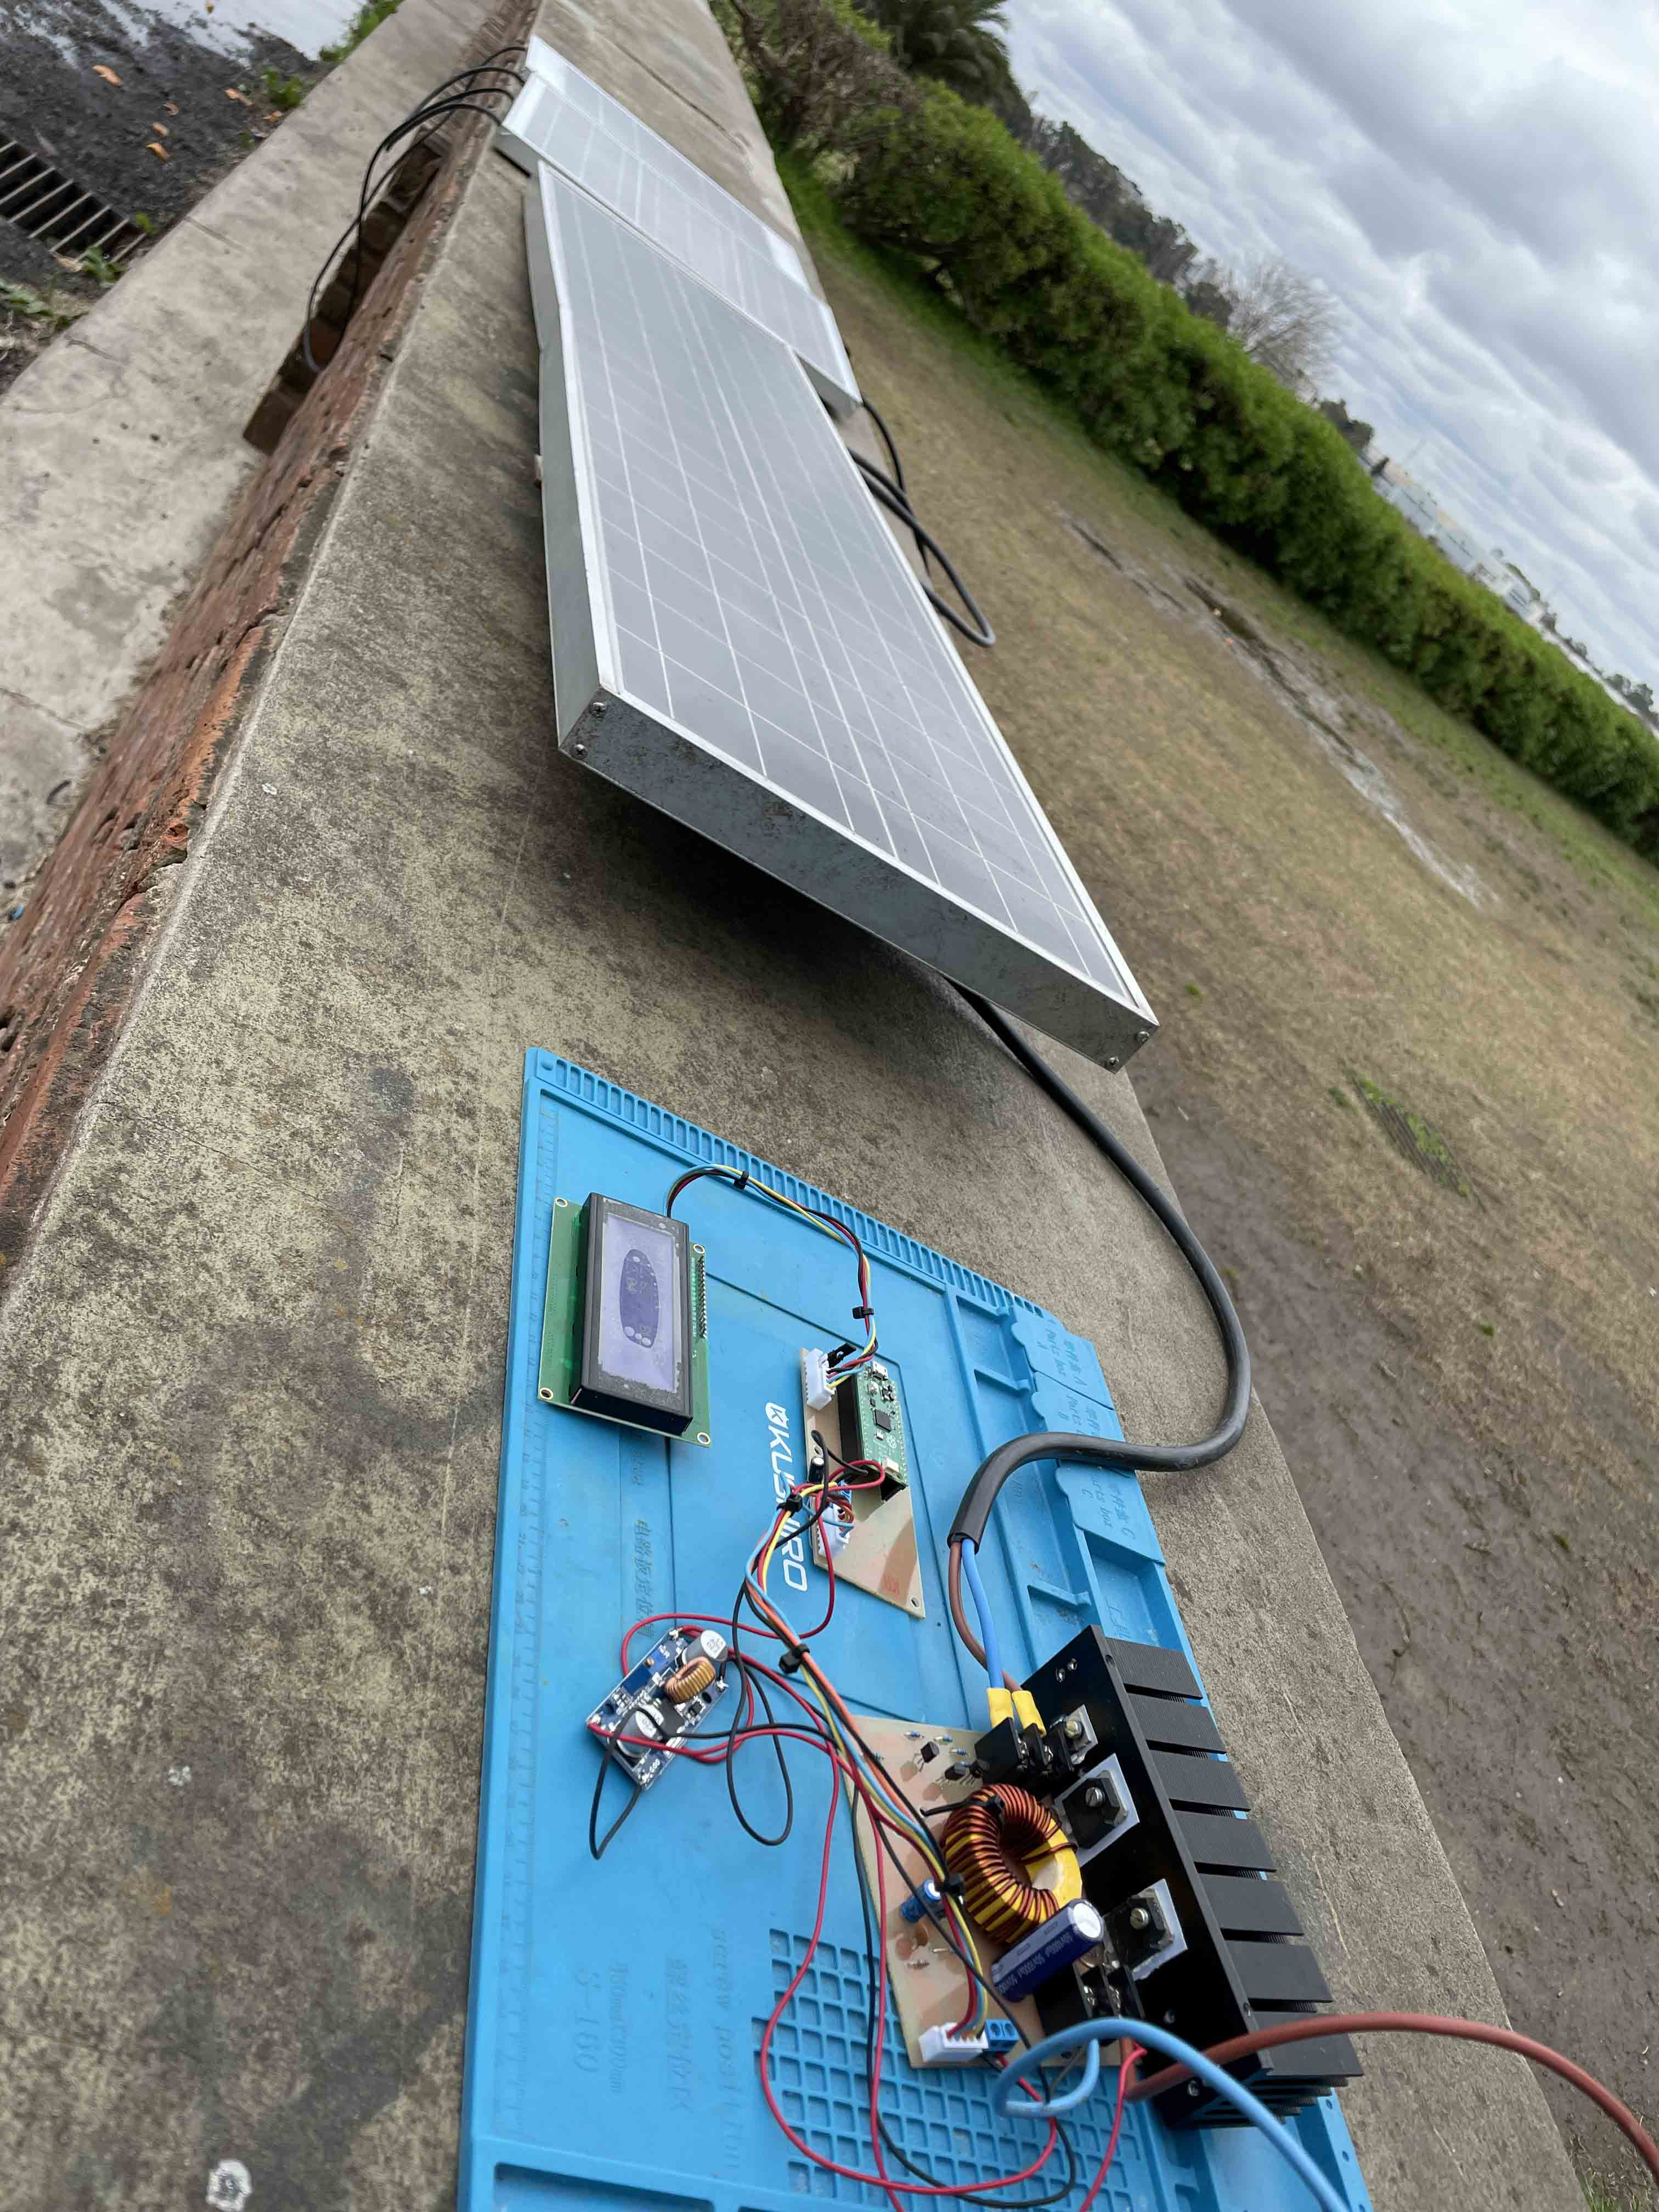
\includegraphics[width=0.9\linewidth]{MPPT/IMG_8913.jpg} 
        \caption{Cargador conectado a paneles\\ solares.}
        \label{fig:paneles-solares-MPPT}
    \end{subfigure}
    \begin{subfigure}{0.5\textwidth}
        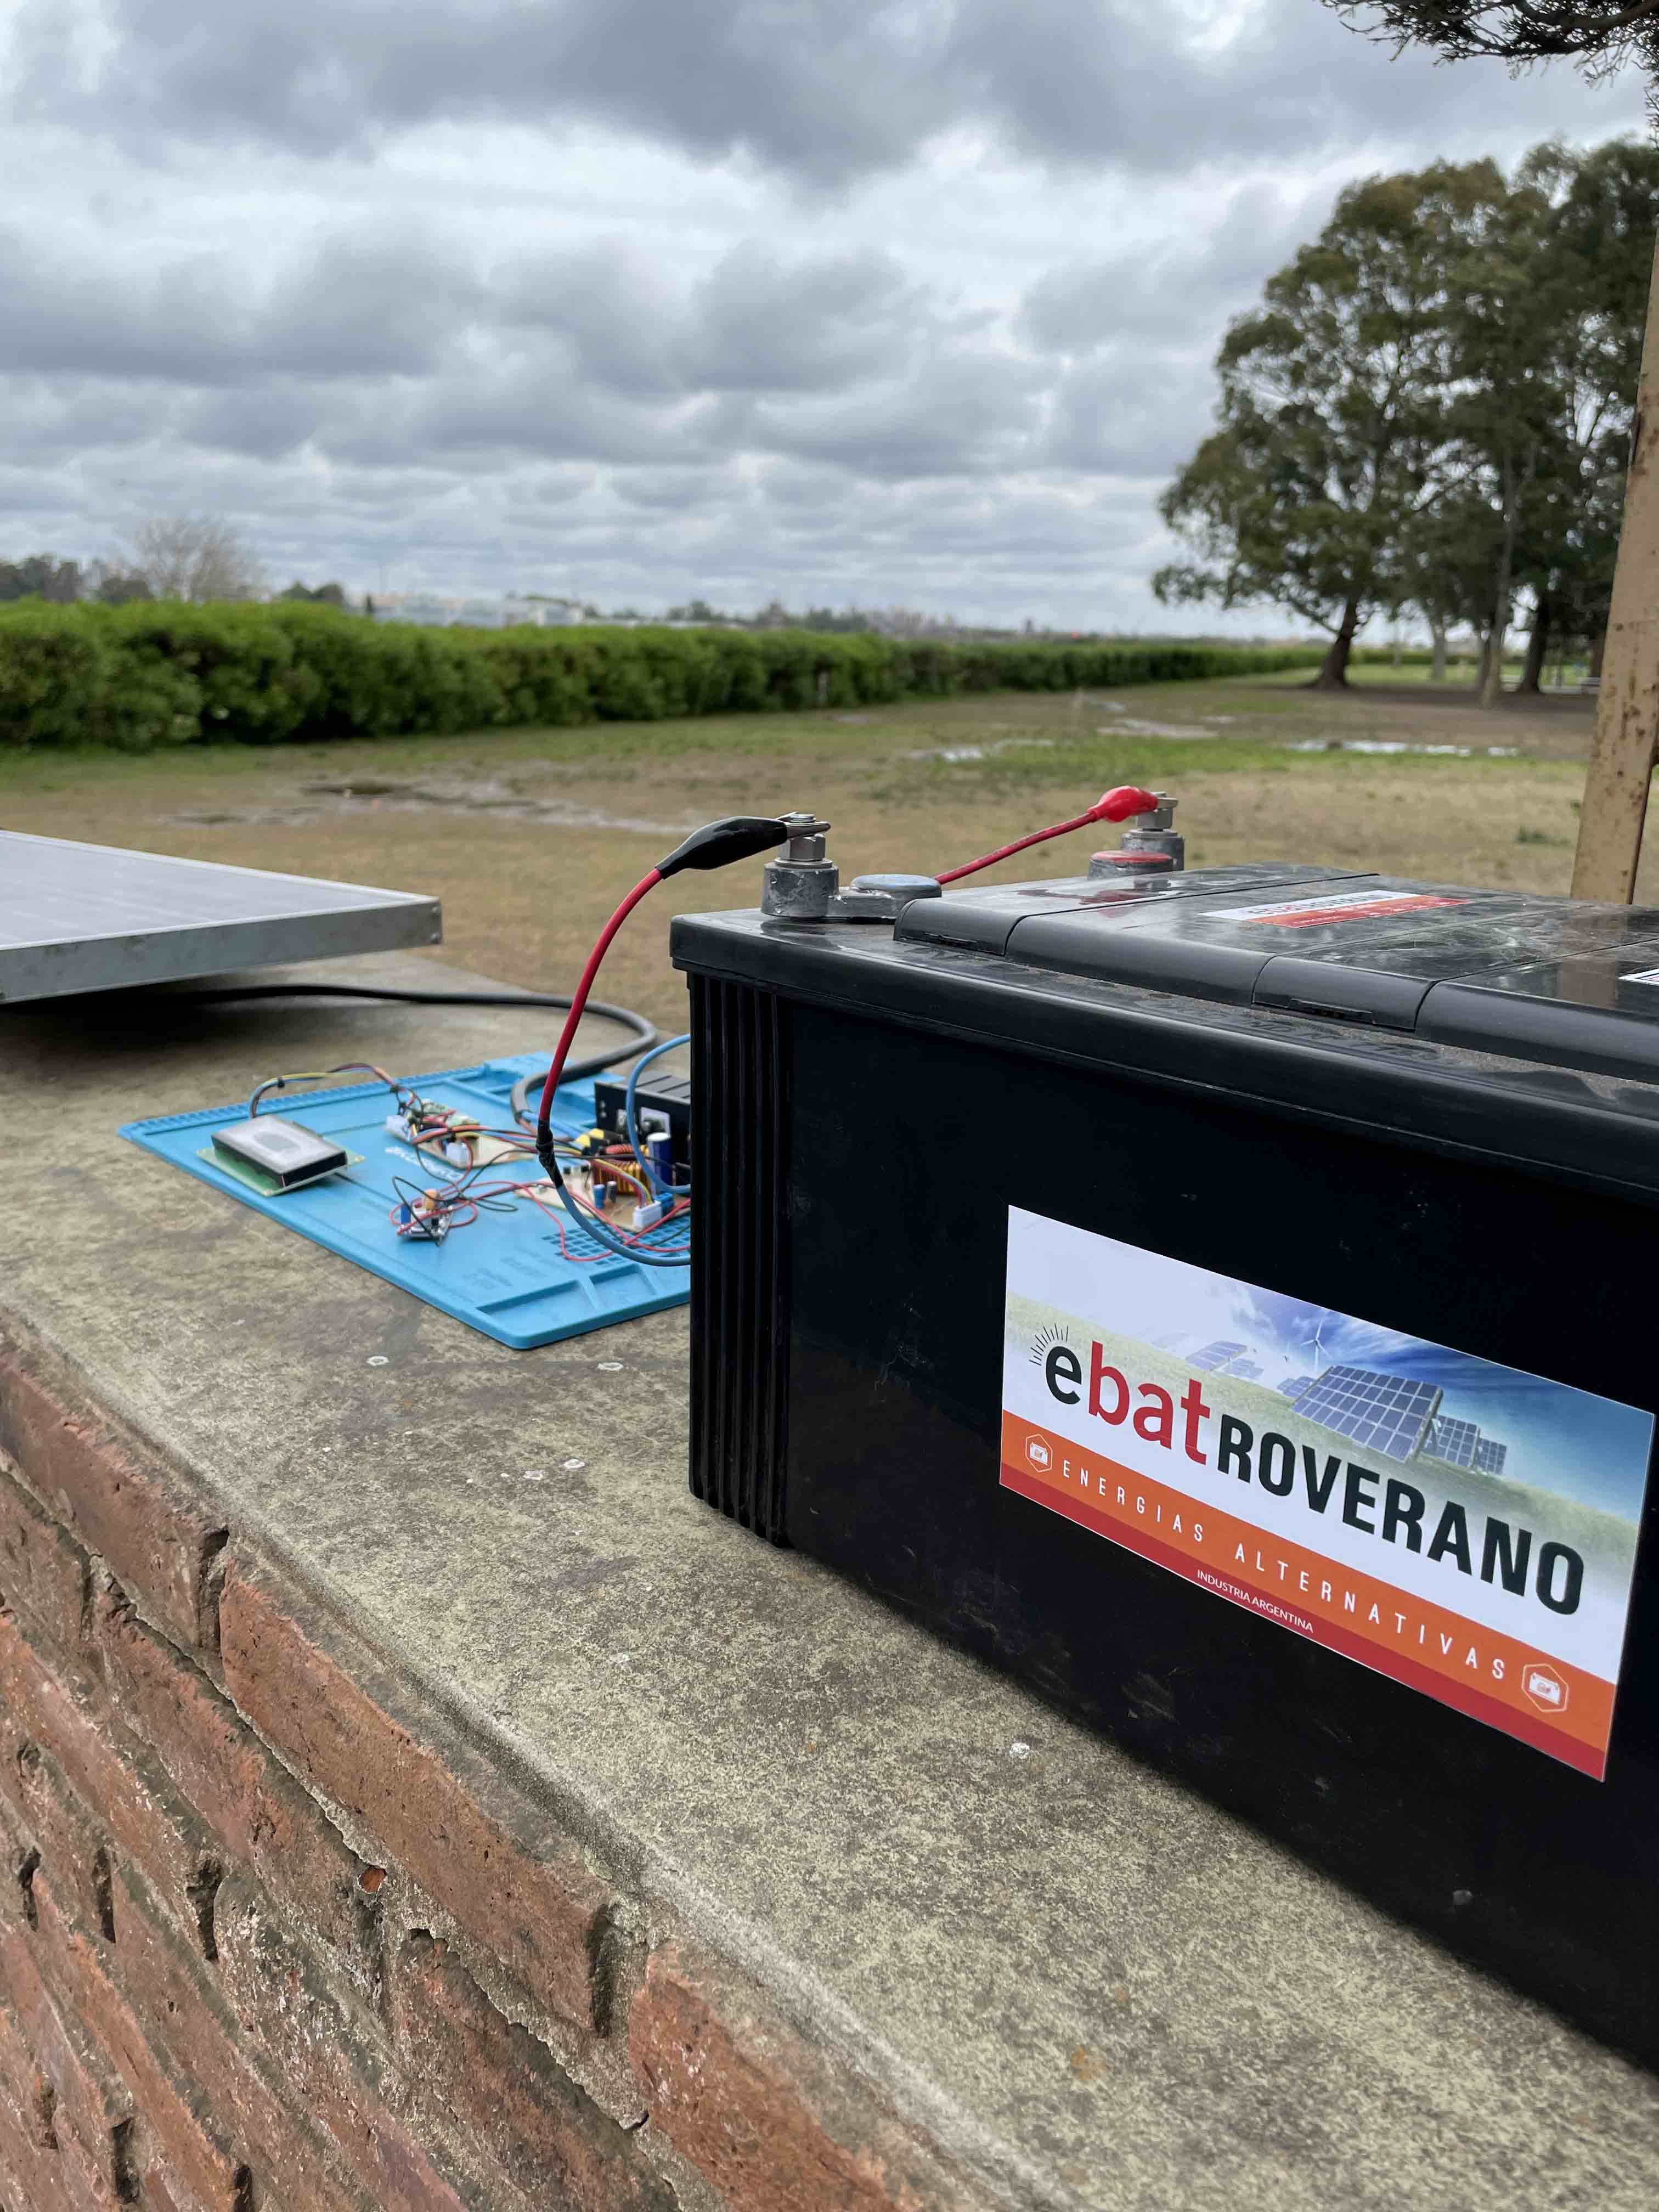
\includegraphics[width=0.9\linewidth]{MPPT/IMG_8915.jpg}
        \caption{Cargador conectado a una batería\\ de ciclo profundo.}
        \label{fig:MPPT-bateria}
    \end{subfigure}
\caption{Cargador MPPT en uso.}
\end{figure}

\begin{figure}[H]
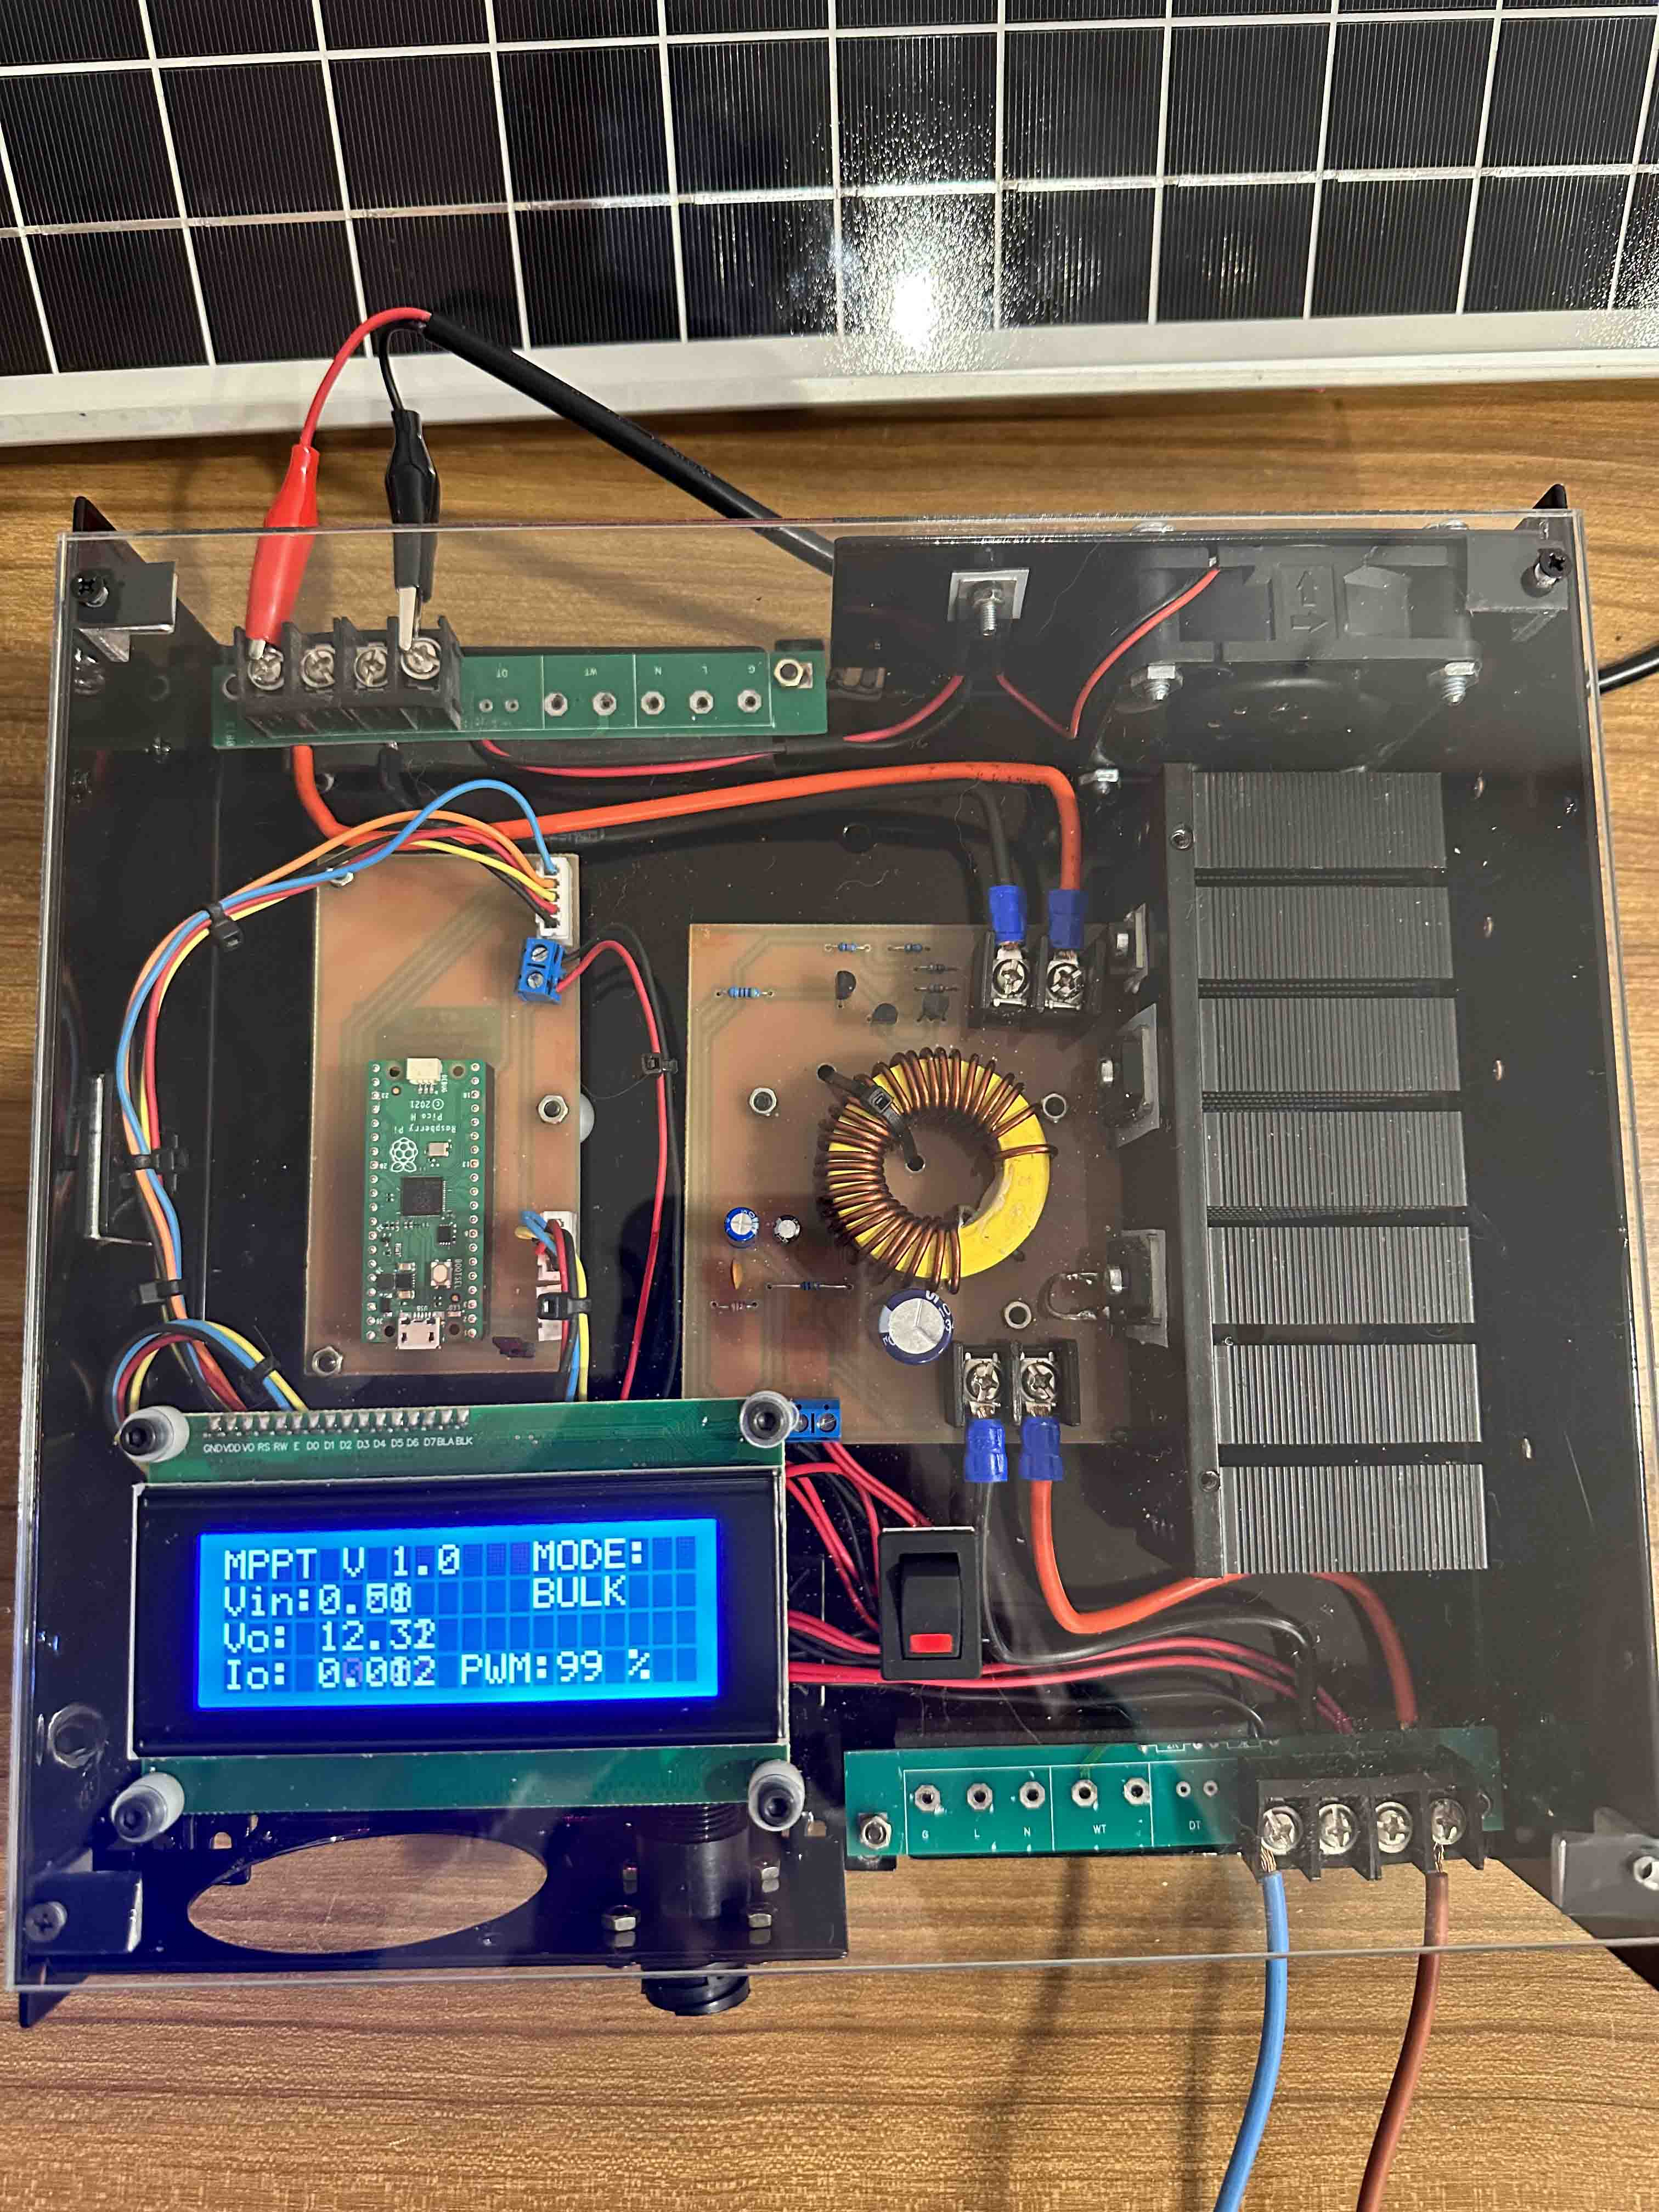
\includegraphics[width=0.9\linewidth]{MPPT/IMG_8032.jpg} 
\caption{Cargador presentado en gabinete.}
\label{fig:MPPT-fin-1}
\end{figure}

\begin{figure}[H]
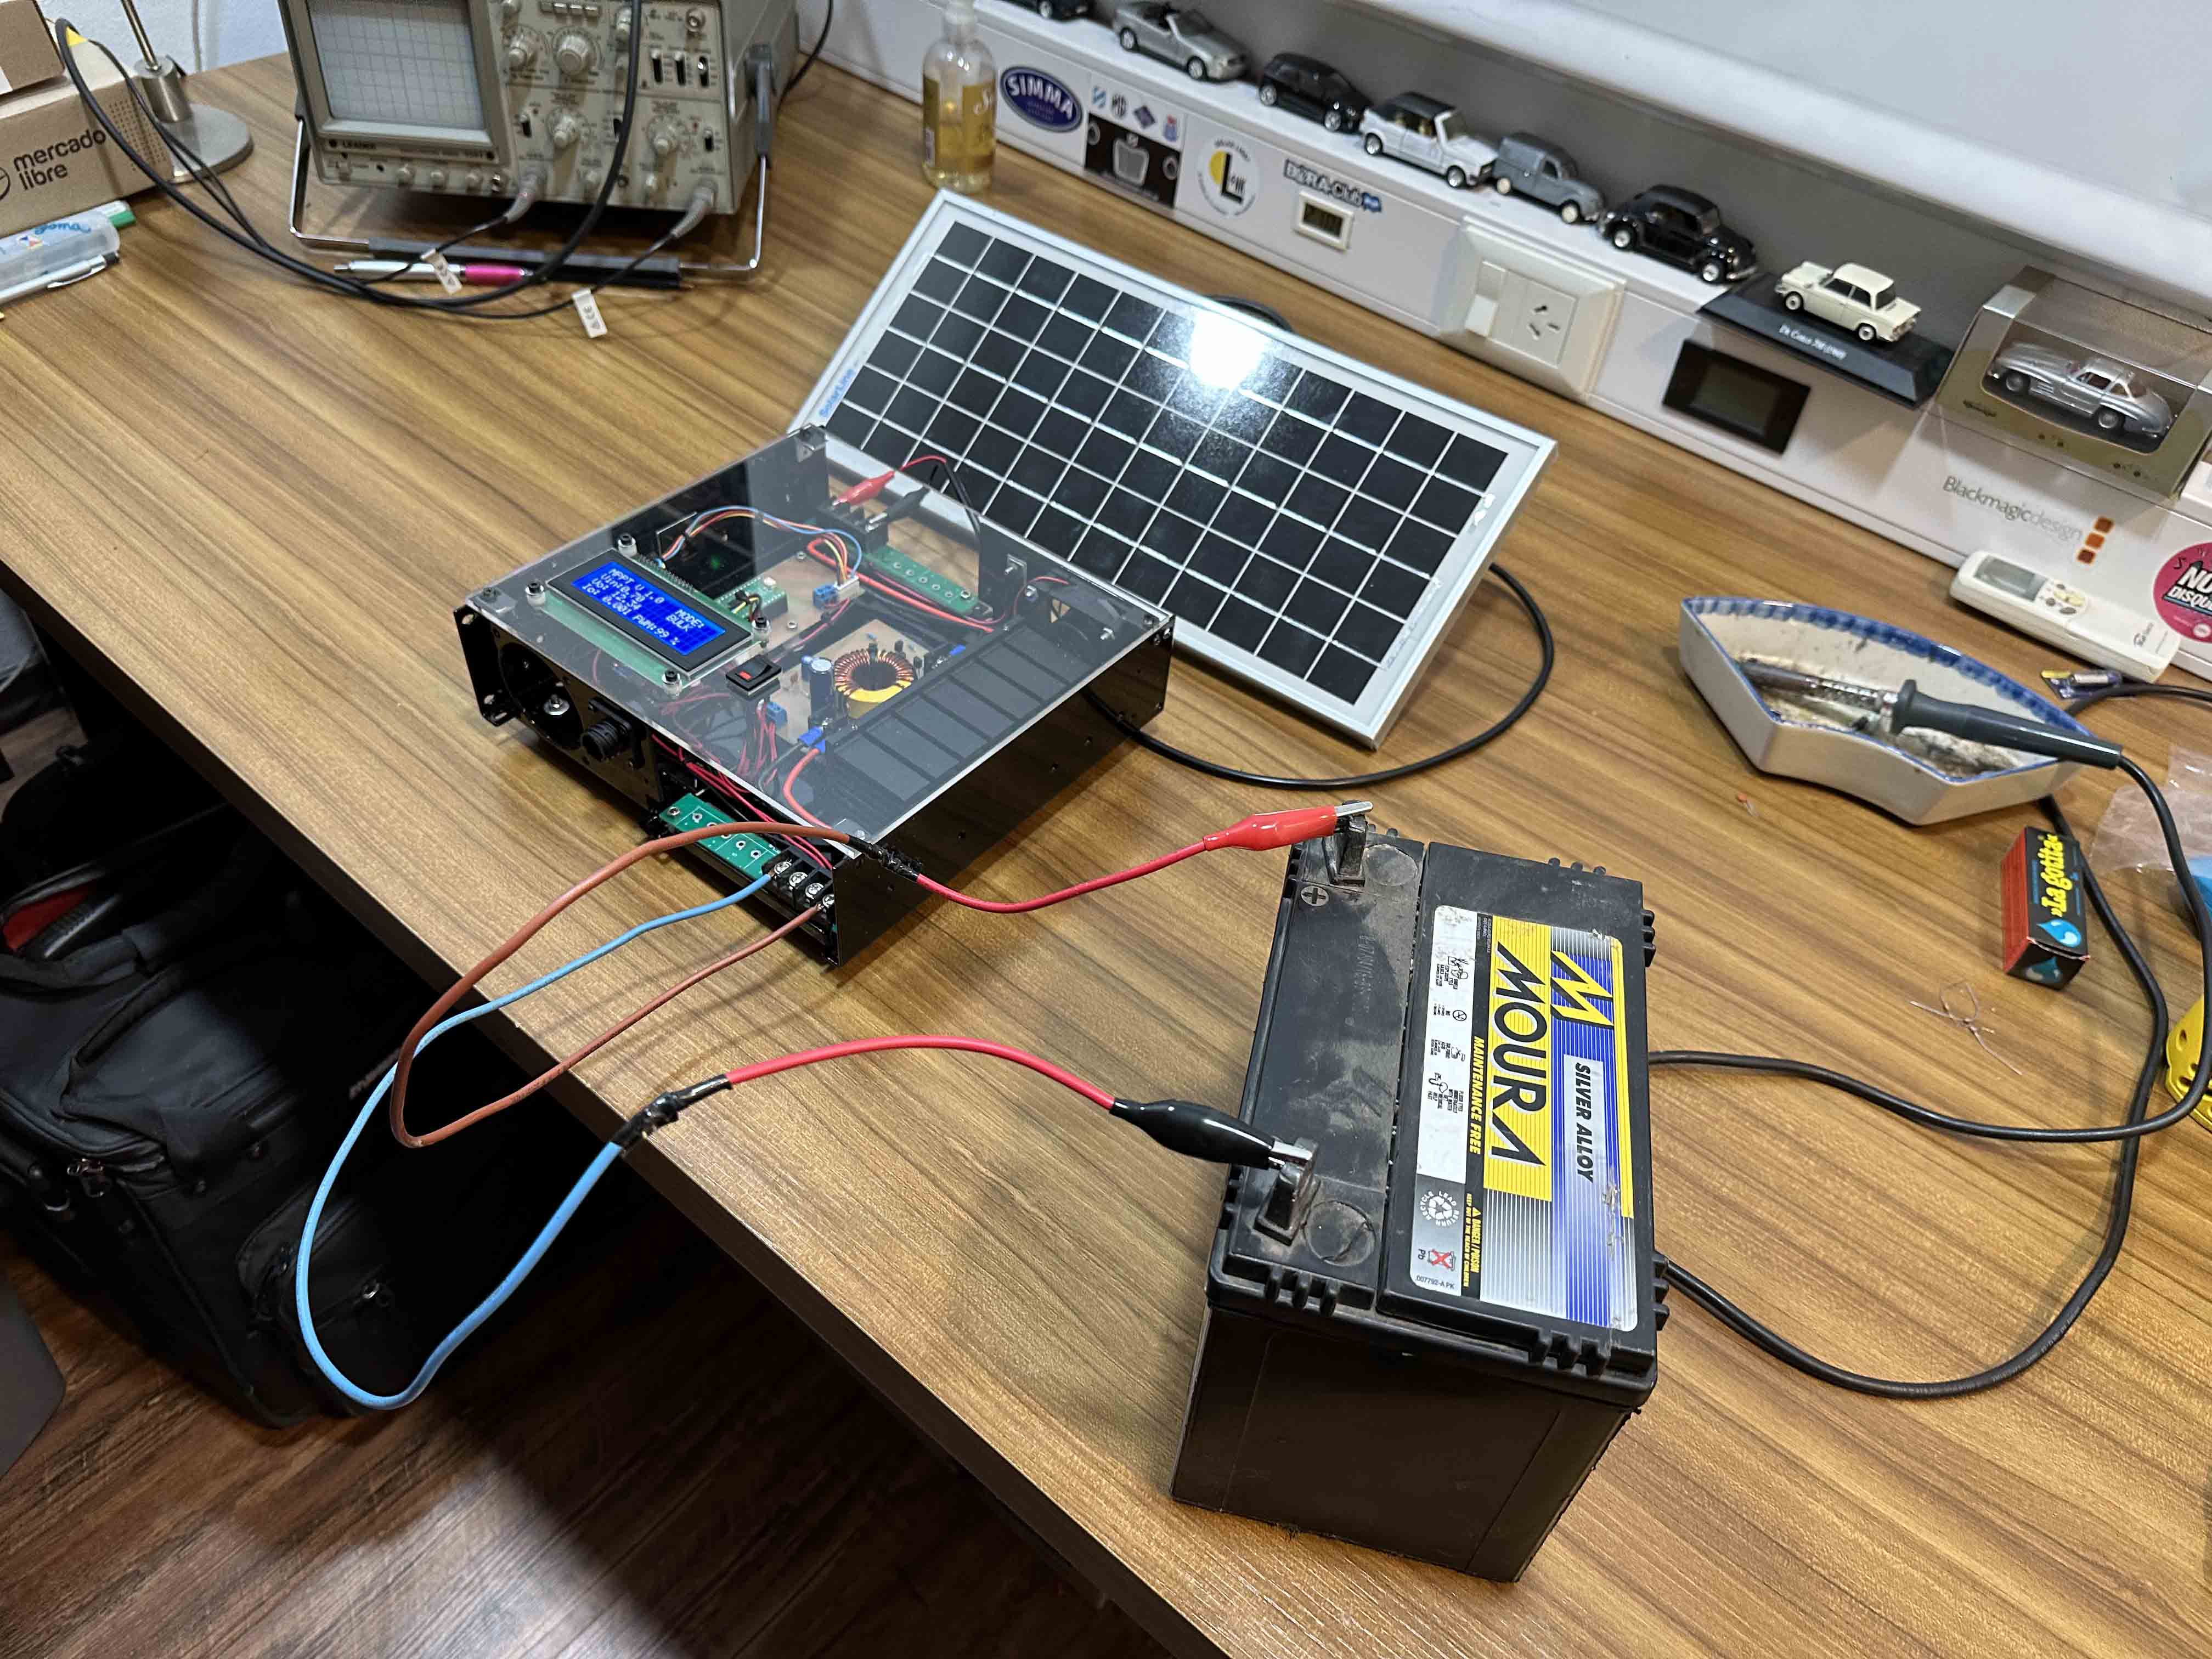
\includegraphics[width=0.9\linewidth]{MPPT/IMG_9390.jpg}
\caption{Cargador en funcionamiento.}
\label{fig:MPPT-fin-2}
\end{figure}

Para su presentación final, se elaboró un gabinete a partir de dos chasis de fuentes switching en desuso, unidas y pintadas, y para la parte superior se utilizó un acrílico para poder ver en su interior. También se le agregó un cooler en la zona del disipador, encargado de extraer calor del gabinete. Este cooler está conectado a traves de otra fuente Step Down a los paneles solares.\\

Como conclusión, se puede decir que es un cargador único en su tipo, aprovechando los últimos avances tecnólogicos para la carga de baterías, logrando una calidad especial en la carga. Este tipo de cargadores que alargan la vida útil de una batería con las 3 etapas de carga, y con una eficiencia por encima del 90\%, no se comercializan actualmente en Argentina.\\

Para finalizar, las mejoras que se pueden realizar en un futuro a este prototipo, se puede agregar un sensor de temperatura para protegerlo frente a un sobrecalentamiento, y un selector de corrientes de carga, siendo que este parámetro es el único que varía realmente entre baterías. De esta forma, quedaría protegido y tendría una opción para cargar diferentes baterías.\\


\subsection{Especificaciones}

Convertidor reductor DC-DC microcontrolado

\begin{itemize}
    \item Voltaje de entrada mínimo: 12Vdc
    \item Voltaje de entrada máximo: 25Vdc
    \item Corriente de entrada máxima: 20A
    \item Voltaje de salida mínimo: 12Vdc
    \item Voltaje de salida máximo: 14,5Vdc
    \item Corriente de salida máxima: 20A
\end{itemize}